In this chapter, we provide simulated and real-world experiments that
demonstrate the robustness properties of the Bayesian framework presented in
Chapter 3.
%
We present three sets of experiments for the Bayesian \textsc{NeuralPbc}
approach.
%
First, we learn a swing-up controller for the simple pendulum and evaluate its
performance under system parameter and measurement uncertainties in simulation.
%
In the second set of experiments, we tackle the swing-up task for the inertia
wheel pendulum and demonstrate the efficacy of the Bayesian controller in
simulation and real-world experiments.
%
Lastly, we demonstrate the performance of the deterministic and Bayesian
\textsc{NeuralPbc} frameworks for hybrid dynamical systems on the rimless wheel,
in simulation and real-world experiments.
%
For the Bayesian \textsc{Neural-IdaPbc} framework, we provide simulated and
hardware experiments for the swing-up task of the IWP.


\section{Bayesian Neural PBC}
\subsection{Simple Pendulum}

In this section, we demonstrate the robustness properties of the controllers
trained via Bayesian \textsc{NeuralPbc} on the simple pendulum system. The system is
simulated under measurement noise via stochastic differential
equations~\eqref{eq:sde_initial}. Furthermore, the system parameter is varied in
order to analyze the closed-loop system response under model uncertainties. 

The equation of motion of a simple pendulum with measurement noise is given by
%
\begin{equation}
    \dd x = \bmat{
        \dot{q} \\ 
        a \sin{(q)} + u^\theta(x)
    } \dd t+ \nabla_x u^\theta(x) \dd W_t,
    \label{eq:pendulum_sde}
\end{equation}
%
where $a=mgl/I$, $\dd W_t$ is the Wiener process, $x = (q,
\dot{q})$ is the state of the pendulum where $q = 0$ corresponds
to the upright position, and the control input $u$ is the torque generated by
the actuator. 
%
The torque \(u^\theta\) is limited by \(\abs{u} \leq u_{\textrm{max}}\).
%
The maximum torque $u_{\textrm{max}}$ available is such that the upward
equilibrium point cannot be reached by just rotating in one direction, as the
gravitational force overcomes the motor torque eventually. The controller has to
be clever enough to overcome gravitational forcing with a combination of
built-up momentum and torque bandwidth.

The objective of this case study is to stabilize the homoclinic orbit of the
pendulum whose single parameter $a$ has the nominal and yet unconfirmed value
$9.81$ \unit{$s^{-2}$}. To this end, we learn a Bayesian control $u^\theta$ that
can stabilize the pendulum even with system parameter uncertainties.

\subsubsection{Training} 
The goal of this training is to track the expert trajectories generated by the
vanilla energy-shaping control (ESC)~\cite{underactuated}. The ESC takes the
general form
%
\begin{equation}
    u^\theta(q, \dot{q}; \theta^e) = \theta^e_1 \dot{q} + \theta^e_2 \cos{(q)} \dot{q} + \theta^e_3 \dot{q}^3,
    \label{eq:pendulum_esc}
\end{equation}
%
where $\theta^e$ represents the parameters of the expert. The weights
$\{\theta^e_i\}_{i=1}^3$ satisfy $-\theta^e_1 = \theta^e_2 = 2a \theta^e_3 < 0$
in the vanilla ESC. 
%
The Bayesian control is also linear over the decision parameters, i.e.
\begin{align*}
    u^\theta(q, \dot{q}; \theta) = \theta_1 \dot{q} + \theta_2 \cos{(q)} \dot{q} + \theta_3 \dot{q}^3,
\end{align*}
and unlike ESC, the learned parameters $\theta$ are samples drawn from the posterior.


The running cost function is chosen to be the loss $J_{track}(\phi_\bot)$ from
homoclinic orbit $\phi^\star$ provided in~\eqref{eq:xperploss}; the
corresponding likelihood is given by~\eqref{eq:track_likelihood}. We collect
dataset $\mathcal{D}_N$ of initial states sampled with greedy and explorative
techniques. For this particular experiment, we use Hamiltonian Monte Carlo
outlined in Algorithm~\ref{algo:hmc} to infer the exact posterior distribution.
We compare the Bayesian policy with the deterministic policy, which is simply
given by the point-estimates of the expert vanilla ESC
in~\eqref{eq:pendulum_esc}~\cite{acc}.

\subsubsection{Simulation Tests} 
The homoclinic orbit of the pendulum is defined by the $2a$-level set of the
total energy $\mathcal{H} = \nicefrac{1}{2}\dot{q}^2 + a(1 +
\cos{q})$. Hence, an appropriate measure of the distance to the
homoclinic orbit is given by the absolute value $\bigl| \mathcal{\tilde{H}}
\bigr|$ of the error: $\mathcal{\tilde{H}} = \mathcal{H} - 2a$. We evaluate the
performance of a closed-loop system by recording the value $\zeta = \min \,
\bigl| \mathcal{\tilde{H}} \bigr|$, where the minimum is taken over the last $2$
seconds of a $10$-second-long trajectory.


We demonstrate the robustness of the Bayesian policy by comparing $\zeta$,
as a function of the system parameter $a$, with that of the deterministic
policy.
%
We also investigate the effects of the prior distribution of $\theta$ on the
performance of the controllers.
%
In particular, we examine a uniform prior and a Gaussian prior centered around
the deterministic solution of~\eqref{eq:pendulum_esc}.
%
The comparisons between the controllers from both cases are shown in
Figure~\ref{fig:bayes_compare}.
%

In addition to uncertainties in $a$, we test the deterministic and Bayesian
policies with measurement noise, modeled as a Wiener process with standard
deviation $0.0005$ \unit{rad} in the $q$-direction and $0.05$ \unitfrac{rad}{s}
in the $\dot{q}$-direction.
%
These numbers are chosen to represent a typical error arising from an
optical encoder with a resolution of 2048 pulses per revolution and its naive
differentiation via backward difference.
%
To capture the influence of measurement noise, we generate 20 trajectories
by integrating~\eqref{eq:pendulum_sde} from the same initial states. 
%
These trajectories are then used to compute $\zeta$. 
%
The effects of noise on $\zeta$ are reflected by the error bands in
Figure~\ref{fig:bayes_compare}.

The results, shown in Figure~\ref{fig:bayes_compare}, demonstrate that Bayesian
learning yields controllers that outperform their deterministic counterpart
throughout the whole range of $a$.
%
The marginalization method in~\eqref{eqn:marginalization} for selecting $\theta$
from the learned distribution performs best when a uniform prior is used, while
the MAP method performs best with the Gaussian prior.
%
We emphasize that the error bands of the marginalized and MAP point
estimates stay well below those of the deterministic curve in the top plot of
Figure~\ref{fig:bayes_compare}.
%
This implies that the controllers produced by Bayesian learning perform
consistently better than the deterministic controller, demonstrating their
robustness against model uncertainty and measurement noise.


\begin{figure}[tb]
    \centering
    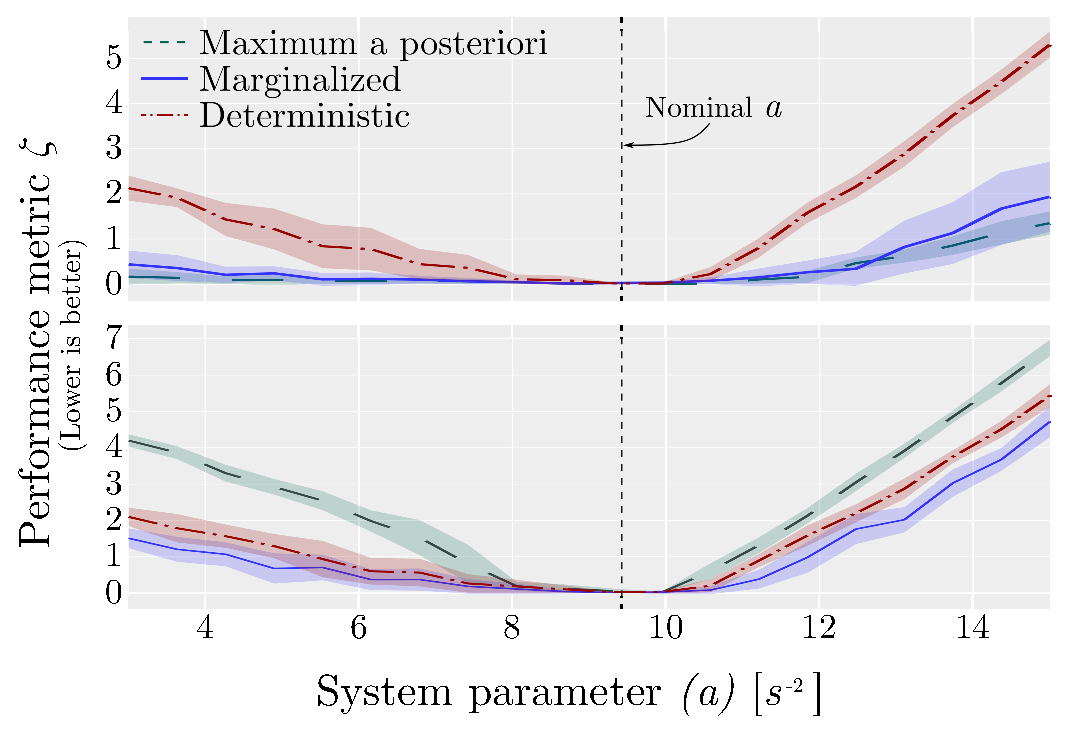
\includegraphics[width=0.8\linewidth]{figures/H_combined.eps}
    \caption{
        Performance comparisons between deterministic and Bayesian learning
        methods. 
        %
        The training is initialized with a Gaussian prior (top), and a
        uniform prior (bottom). 
        %
        The continuous error band is generated by computing $\zeta$ from 20
        trajectories of~\eqref{eq:pendulum_sde}, starting at the downward
        equilibrium with a small disturbance. 
        %
        The solid lines represent the mean of $\zeta$. 
        %
        Best viewed in color.
        %
    }
    \label{fig:bayes_compare}
\end{figure}
%%%%%%%%%%%%%%%%%%%%%%%%%%%%%%%%%%%%%%%%%%%%%%%%%%%%%%%%%%%%%%%%%%%%%%%%%%%
\subsection{Inertia Wheel Pendulum}
\label{subsec:iwp}
In this section, we validate the Bayesian \textsc{NeuralPbc} framework on the
problem of swinging-up and stabilizing the inverted position of an inertia wheel
pendulum (IWP), shown in Fig.~\ref{fig:iwp}. We provide experimental results
from simulation and real-world hardware in order to thoroughly demonstrate the
efficacy and robustness claims of Bayesian inference. 
%
We use the deterministic solution for \textsc{NeuralPbc} as the baseline on
which we compare the performance of the Bayesian solution. 

\subsubsection{System Model}

The IWP mechanism consists of a pendulum with an actuated wheel instead of a
static mass.
%
The wheel has mass $m$, which is connected to a massless rod of length \(l\). 
%
The position of the rod is denoted by the angle \(q_1\) measured with
respect to the downward vertical position.
%
The position of the wheel \(q_2\) is measured with respect to the vertical
line through the center of the wheel.
%
The Hamiltonian of the IWP is given by Equation~\eqref{eq:system_hamiltonian}, where
%
\begin{equation*}
    M = \bmat{I_1 & 0 \\ 0 & I_2},
    \;
    G = \bmat{-1 \\ \phantom{-}1},
    \;
    V(q) = mgl \left( \cos q_1 - 1 \right),
\end{equation*}
%
and $p = \left(I_1 \dot{q}_1,I_2 \dot{q}_2\right)$. 
%
We denote the state of the system as $x = (q_1, q_2, \dot{q}_1, \dot{q}_2)$.
%
The parameters \(I_1\) and \(I_2\) denote the moment of inertia of the pendulum
and the wheel, respectively, and \(g\) is the gravitational constant.
%
The equations of motion of the IWP with measurement noise can be written as 
%
\begin{equation}
    \dd x = \bmat{\dot{q}_1 \\ \dot{q}_2 \\ \dfrac{mgl \sin(q_1) - u^\theta - b_1\dot{q}_1}{I_1} \\ \dfrac{u^\theta - b_2 \dot{q}_2}{I_2}} \dd t + \nabla_x u^\theta(x) \dd W_t, 
    \label{eq:iwp_dynamics}
\end{equation}
%
where the control input \(u^\theta\) is the torque applied to the inertia wheel
and $\{b_i\}_{i=1}^2$ are friction coefficients.
%
The desired equilibrium $x^\star$ is the origin, which corresponds to the upward
position.
%
The nominal system parameters are estimated to be $I_1 = 0.0455$ kg-m$^2$, $I_2
= 0.00425$ kg-m$^2$, and $mgl = 1.795$ N-m. 
%
% The control objective is to ensure that closed-loop trajectories
% of~\eqref{eq:iwp_dynamics} passes through a neighborhood of $x^\star$,
% at which point a linear stabilizing controller can be employed to asymptotically
% stabilize the system at $x^\star$.
%

\begin{figure}[t]
    \centering
    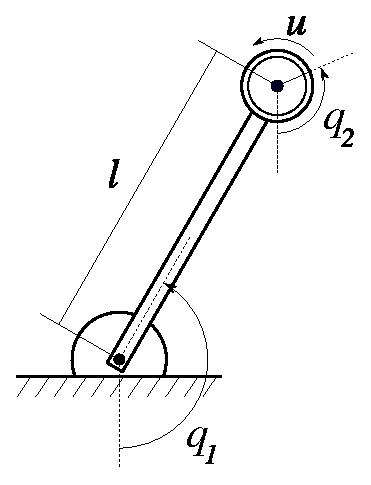
\includegraphics[width=0.25\linewidth]{figures/iwp.eps}
    \caption{Schematic of the inertia wheel pendulum. Only the joint $q_2$ is actuated, and $q_1$ is not.}
    \label{fig:iwp}
\end{figure}

\subsubsection{Training} 

The energy-like function $H_d^\theta$ is a fully-connected neural network with
two hidden layers, each with the \textsc{Elu} activation
function~\cite{clevert2015fast}. 
%
% There are, in total, 137 parameters to learn. 
% %
% They are initialized according to the Glorot
% (Xavier)~\cite{glorot2010understanding} scheme.
%
% The objective of the optimization problem~\eqref{eq:neural_pbc_finite_optim}
% consists of $\ell_{\textrm{set}}$ given by Equation~\eqref{eq:set_distance},
% with the set $\mathcal{S}$ chosen as a ball of radius $r = 0.01$ around
% $x^\star$ in the standard norm topology.
%
A uniform distribution in $[-2\pi, 2\pi] \times [-2\pi, 2\pi] \times [-10, 10]
\times [-10, 10]$ is chosen as the probability distribution from which samples
of initial states $x_0$ are drawn for the \textsc{DAgger} strategy.
%
In each gradient descent step, we sample a batch of 4 initial states $\{x_0\}$
from greedy and explorative state sampling techniques; these initial states are
integrated forward with a time horizon of $t \in [0,3]$ seconds. 
%
In the Bayesian framework, the standard deviations $\sigma_{p}$ of system
parameters $p_s = [I_1, I_2, mgl]$ are chosen to be $10\%$ of the nominal system
parameters.
%
Moreover, we train on trajectories per the SDE in~\eqref{eq:sde_initial} with
measurement error represented by Wiener process with standard deviation of 0.001
and 0.02 on the joint angles and velocities, respectively.
%
% In each gradient descent step, a batch of 4 initial conditions $\{x_0\}$
% generated by \textsc{DAgger} is integrated forward with using the Tsitouras
% $5(4)$ Runge-Kutta solver with a time horizon of $t \in [0,3]$ seconds. 
%
% The cost function is then computed and back-propagated using the
% AD-assisted adjoint method implemented in
% \verb|DiffEqFlux.jl|~\cite{DBLP:journals/corr/abs-2001-04385}.
% %
% In the Bayesian learning framework, we draw samples from the posterior and
% back-propagate through the gradients of the \textsc{Elbo} using the
% \textsc{ADVI}~\cite{kucukelbir2015automatic} scheme provided in
% \verb|Turing.jl|~\cite{turing}. 
%

We use variational inference to estimate a Gaussian posterior distribution
over uncorrelated parameters. The trainings are terminated when the loss
function $J(\gamma) = J_{set}(\gamma) + J_T(\gamma)$ and the \textsc{Elbo}
converge for the deterministic and Bayesian trainings, respectively.
%
The hyperparameters for the deterministic and Bayesian \textsc{NeuralPbc}
trainings are shown in Table~\ref{tab:training_setup_neuralpbc}.
%
It can be seen that the Bayesian training effectively learns with smaller
neural network size than the deterministic training.
\begin{table}[tb]
    \centering
    \caption{\textsc{NeuralPBC} training setup for deterministic and Bayesian frameworks}
    % \rowcolors{2}{}{Wheat1}
    \begin{tabular}{lcc}
    \toprule
    %   & \multicolumn{2}{c}{Framework} \\
    %   \cmidrule(lr){2-3}
    & Deterministic & Bayesian \\
    \midrule
        $H_d$ neural net size & (6, 12, 3, 1) & (6, 5, 3, 1)\\
        Learned parameters & 133 & 128  \\
        Optimizer & \textsc{ADAM} & DecayedAdaGrad\\
        Initial learning rate & 0.001 & 0.01\\
        Replay buffer size & 400 & 50\\
    \bottomrule
    \end{tabular}
    \label{tab:training_setup_neuralpbc}
\end{table}

\subsubsection{Simulation Tests} 
The performance of the controllers obtained from the deterministic and Bayesian
trainings are compared as follows.
%
We evaluate the performance of both trainings with parameter uncertainties
on $I_1, I_2$ and $mgl$. 
%
We introduce these uncertainties by moving the average
system parameters by $\pm 10\%$ to $\pm 50\%$ with increments of $10\%$. 
%
For each average system parameter, we sample uniformly with a $\pm 5\%$ support
around the average system parameters. 
%
This helps test the performance of the controller with various combinations of
$I_1, I_2$ and $mgl$.
%
On top of the system parameter uncertainties, we introduce measurement noise
represented by a Wiener process with standard deviation of $0.001$ and $0.02$ on
the joint angles and velocities, respectively. 
%
Figure~\ref{fig:comparison_neuralpbc} shows the performance of deterministic and
Bayesian trainings using an accumulated quadratic loss of the form
\begin{equation} J^T = \frac{1}{2}\int_0^T \left(x^\top \mathcal{Q}x + u^\top \mathcal{R}u \right) dt.
\label{eq:performance_metric} \end{equation}
%
The controller learned from the Bayesian training is marginalized over 10
parameters sampled from the posterior.
As seen in Figure~\ref{fig:comparison_neuralpbc}, the Bayesian training
effectively collects less cost for large error in system parameters.
%
Moreover, the error band on the cost of the Bayesian training is smaller than
that of the deterministic training; this shows that the marginalized controller
is more robust against measurement noise.
%   
\begin{figure}[tb]
    \centering
    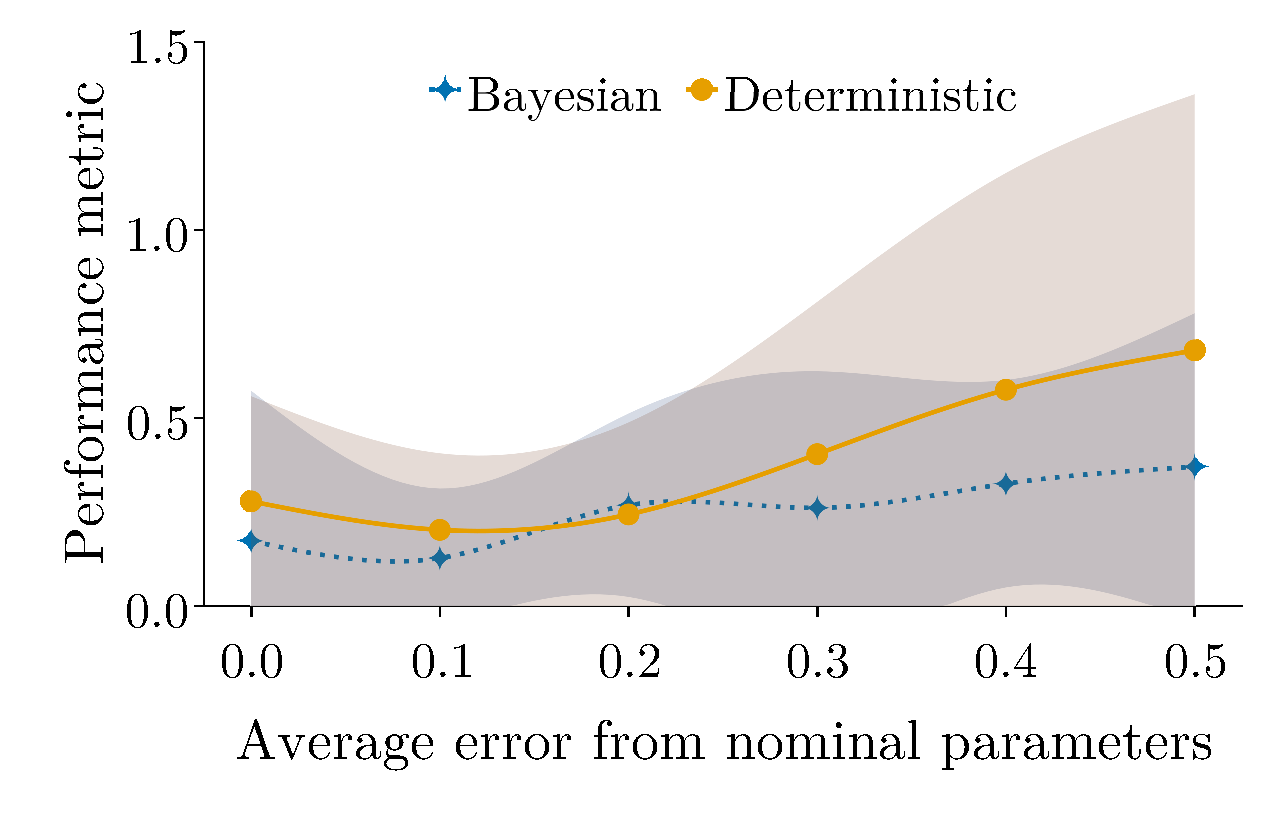
\includegraphics[clip,width=0.7\linewidth]{./figures/bandplot2.eps}%
    \caption{\textsc{NeuralPBC} Performance metric ($J^T$) for various
    error in system parameters. Measurement noise included as Wiener process
    with standard deviation of $0.001$ and $0.02$ on joint angles and
    velocities, respectively}
    \label{fig:comparison_neuralpbc}
\end{figure}

\subsubsection{Hardware Tests} 

The controllers from deterministic and Bayesian training schemes are
evaluated on the hardware shown in Figure~\ref{fig:iwp_hardware}. 
%
We deliberately modify the hardware and test the controllers without any
additional training.
%
In particular, throughout the experiments, the inertia wheel attached to $q_2$
is replaced with parts (labelled A-C on Table~\ref{tab:modified_params}) whose
mass and inertia are different from the nominal values.
%
The modified system parameters are summarized in
Table~\ref{tab:modified_params}.
%
% The parameter error listed on the last column of Table~\ref{tab:modified_params}
% is computed by $\|p - p_{\textrm{nom}}\| / \|p_{\textrm{nom}}\|$.
\begin{table}[H]
    \centering
    \caption{System parameters used in real-world experiments. The errors in the
    last column are $\|p_s - \hat{p}_s\| / \|\hat{p}_s\|$}.
    % \rowcolors{2}{}{Wheat1}
    \begin{tabular}{lcccc}
    \toprule
    Parameter set $p_s$ & $I_1$ & $I_2$ & $mgl$ & Error \\
    \midrule
    Nominal & 0.0455 & 0.00425 & 1.795 & 0 \\
    A & 0.0417 & 0.00330 & 1.577 & $0.122$ \\
    B & 0.0378 & 0.00235 & 1.358 & $0.243$ \\
    C & 0.0340 & 0.00141 & 1.140 & $0.365$ \\
    \bottomrule
    \end{tabular}
    \label{tab:modified_params}
\end{table}
\begin{figure}[tb]
    \centering
    
\includegraphics[width=0.55\linewidth]{hardware.eps}
    \caption{Inertia Wheel Pendulum Hardware}
    \label{fig:iwp_hardware}
\end{figure}

The system starts from rest at the downward position. 
%
A small disturbance in the $q_1$ direction is introduced to start the swing-up.
%
The state $x$ is recorded and~\eqref{eq:performance_metric} is the
performance metric used to evaluate the controllers. The results are
summarized in Figure~\ref{fig:neuralpbc_bar_plot}.
%

In all scenarios, our controllers are able to achieve the control objective
despite the errors introduced in the system parameters.
%
% Furthermore, the controller from Bayesian training consistently outperforms the
% controller from deterministic training, supporting the theoretical justification
% discussed in Section~\ref{ssec:justification}. 
%
These results demonstrate that our approach enables a unified way to tackle
nonlinear control problems while simultaneously incorporating prior knowledge
and model uncertainties.
%
\begin{figure}[H]
    \centering
    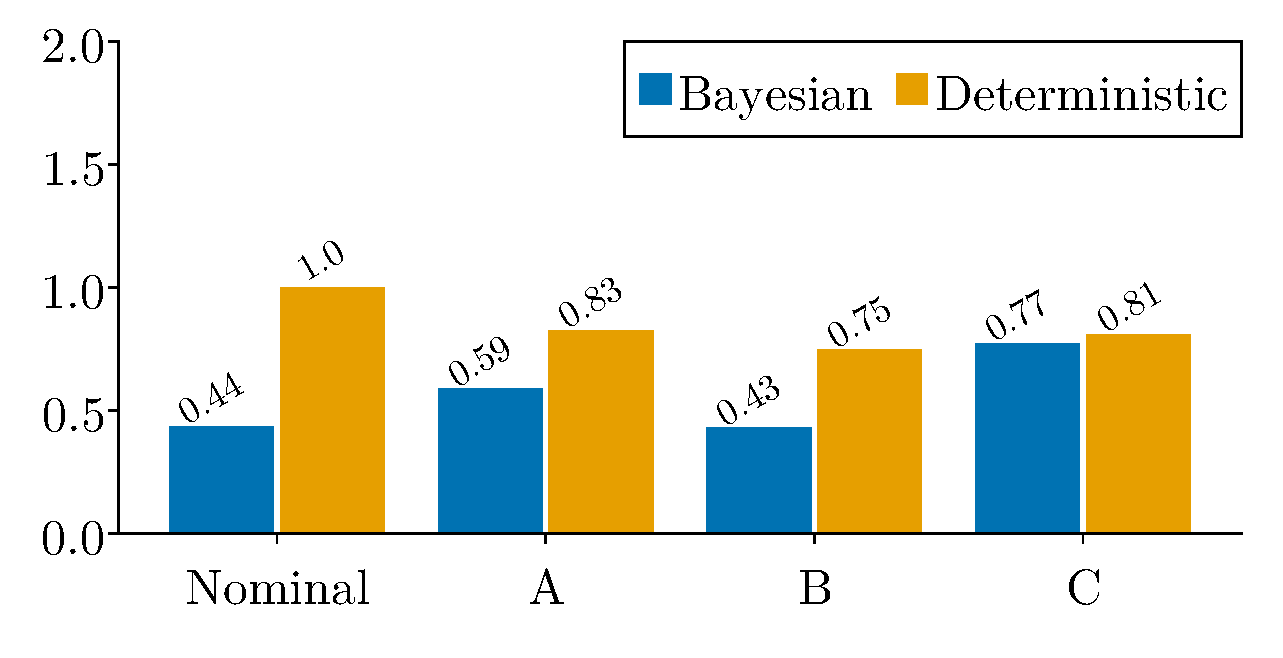
\includegraphics[width=0.7\linewidth]{./figures/pbc_bar.eps}
    \caption{
        %
        Controller performance for modified system parameters. 
        %
        The performance metric is given by
        Eq.~\eqref{eq:performance_metric}.
        %
        Lower values are better. 
        %
        These results show that controllers trained via Bayesian learning are
        consistently more robust to errors in system parameters.
        %
    }
    \label{fig:neuralpbc_bar_plot}
\end{figure}
%%%%%%%%%%%%%%%%%%%%%%%%%%%%%%%%%%%%%%%%%%%%%%%%%%%%%%%%%%%%%%%%%%%%%%%%%%%%%%%%%%%

\subsection{Rimless Wheel}
\label{sssec:rimless_wheel_model}

This mechanism consists of a rimless wheel in the plane with a set of $N$ spokes
and a torso freely rotating about a pin joint located at the center of the
wheel.
% 
The mass of the wheel $m_1$ is concentrated at the hip and spans a radius of
$l_1$.
%
The torso has its mass $m_2$ concentrated at a distance of $l_2$ from the hip. 
%
We actuate the torso angle with the motor mounted at the hip, which in turn
propels the entire wheel forward or back. 
%
The angle of the torso is characterized by $\varphi$ measured from the outward
normal of the runway shown as $\hat{n}$ in Figure~\ref{fig:rimless_wheel_w_torso}.  
%
The orientation of the wheel $\beta$ is measured from $\hat{n}$ to a datum spoke.
%
\begin{figure}
    \centering
    \begin{tikzpicture}
    
        \node [](image) at (0,0) {
            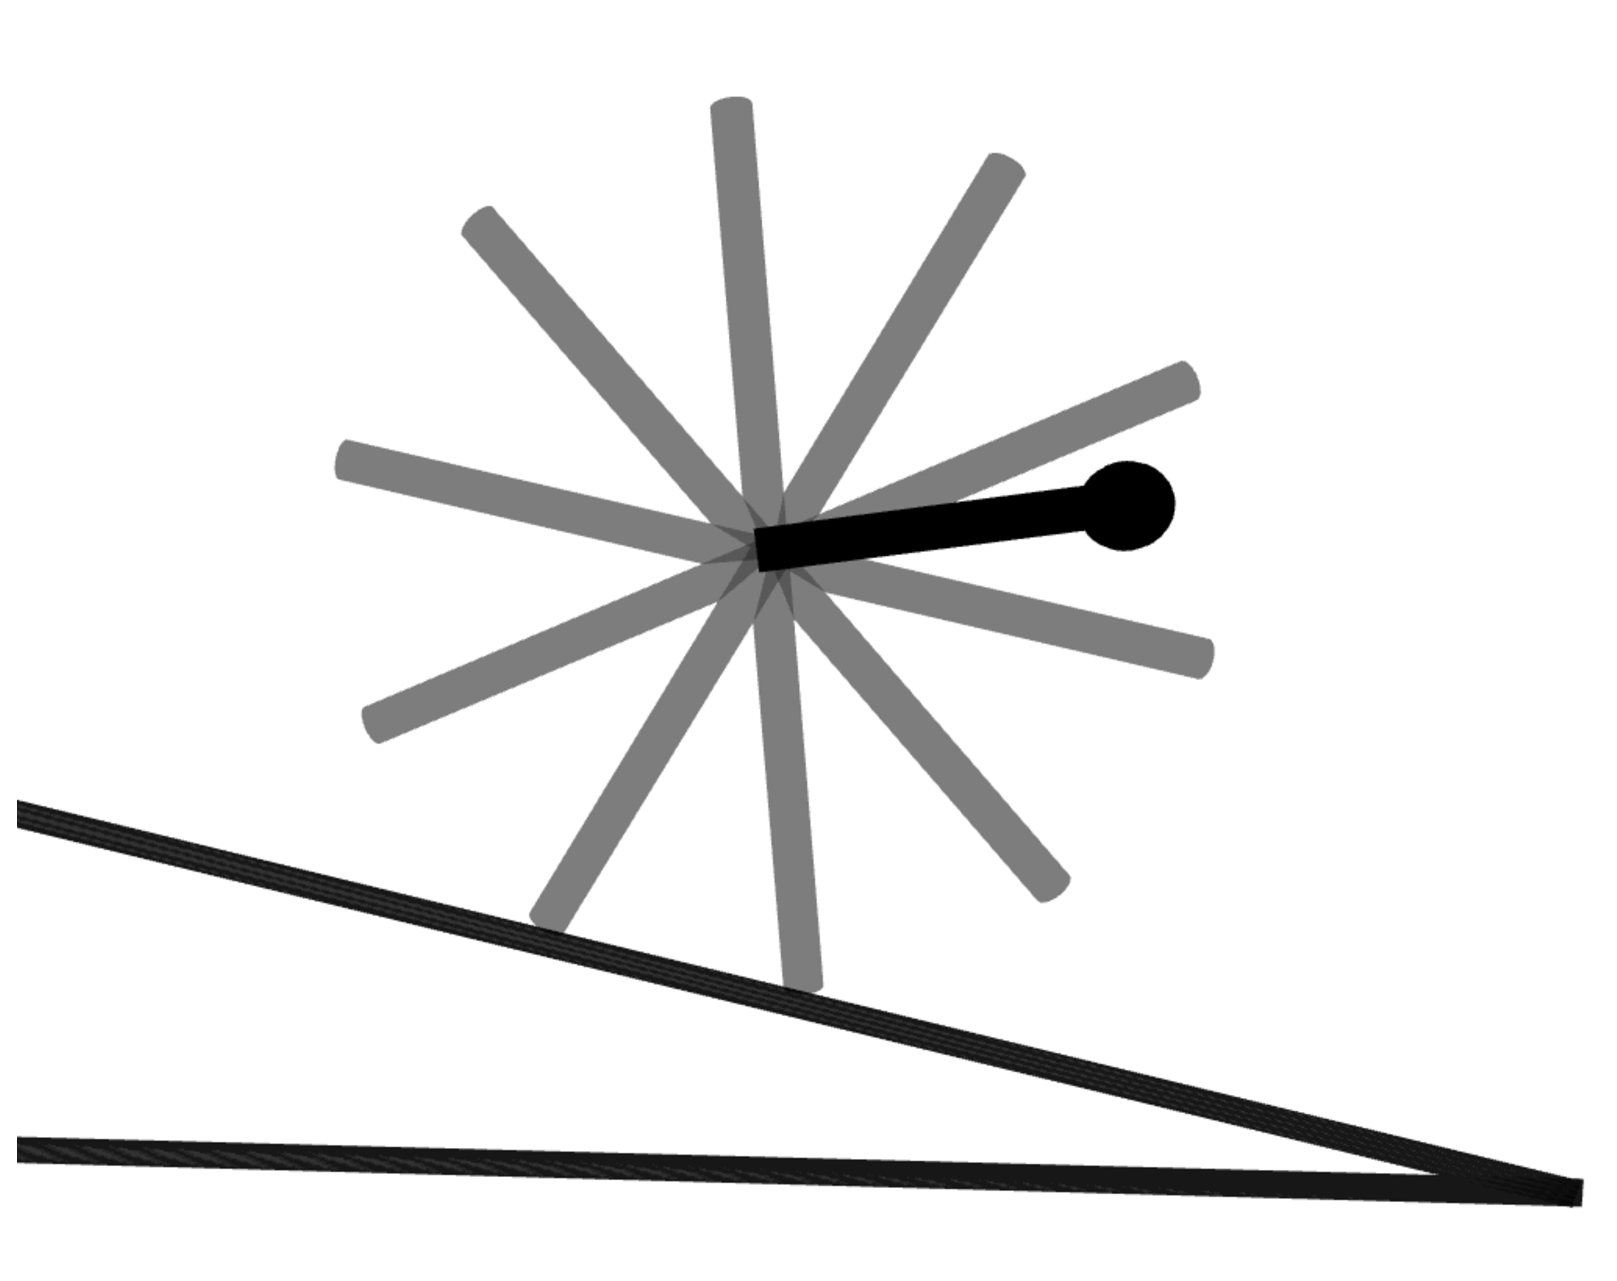
\includegraphics[width=0.5\textwidth]{rimlesswheel.eps}
        };
        \draw[-stealth, very thick,black] (-0.22,0.22) -- ++(-1.7,1.9) node[left,black,fill=white]{\small $l_1$};
        \draw[-stealth, very thick,black] (-0.4,1.9) -- ++(-0.6,0.7) node[above,black,fill=white]{\small $m_1$};
        \draw[-stealth, very thick,black] (1.5,0.8) -- ++(1.0,-0.6) node[right,black,fill=white]{\small $m_2$};
        \draw[-stealth, very thick,black] (-0.24,0.8) -- ++(1.9,0.25);
        \node[black,fill=white] at (1.1,1.5){\small $l_2$};
        % \draw[-stealth, very thick,black] (3.0,-2.6) -- ++(0.3,1.0) node[below right,black,fill=white]{\small $\hat{n}$};
        \draw[-stealth, very thick,black] (-4.0,0.0) -- ++(1.0,-0.3) node[below,black,fill=white]{\small $x$};
        \draw[-stealth, very thick,black] (-4.0,0.0) -- ++(0.3,1.0) node[above left,black,fill=white]{\small $y$};
        \node[below right,black,fill=white] at (-4.8, 0.2) {\small $\Sigma_1$};
        \draw[-stealth, very thick,black]  (2.0,-2.8) arc (180:160:1.0); 
        \node[] at (1.3,-2.5) {\small $\gamma$};
        \draw[-stealth, dotted, very thick,black] (-0.7,-1.8) -- ++(1.2,5.0) node[above right,black,fill=white]{\small $\hat{n}$};
        \draw[-stealth, very thick,black]  (-0.4, -0.5) arc (270:360:1.0); 
        \node[] at (0.8, -0.1) {\small $\varphi$};
        \draw[-stealth, very thick,black]  (0.1, 1.5) arc (90:225:1.0); 
        \node[] at (-1.1, -0.3) {\small $\beta$};
    \end{tikzpicture}
    \caption{Rimless wheel with torso; depicted with $N=10$ spokes.}
    \label{fig:rimless_wheel_w_torso}
\end{figure}
% \begin{figure}[b]
%  \centering
%  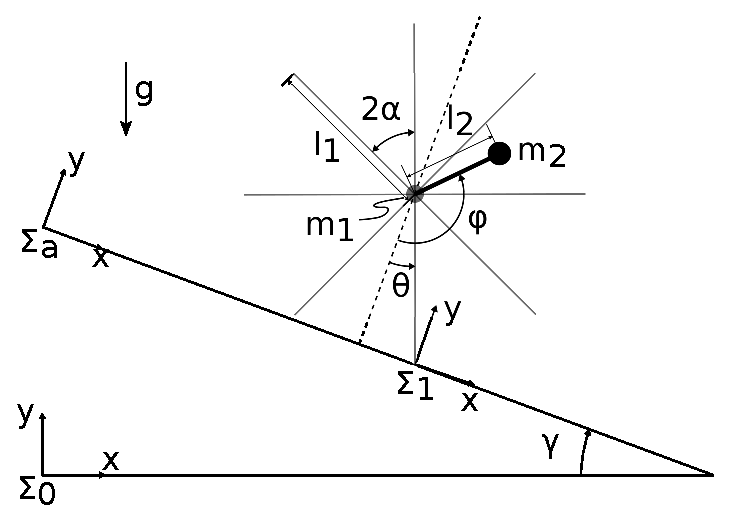
\includegraphics[width=0.75\columnwidth]{./figures/rimless_wheel_with_torso_v3.eps}
%  \caption{Rimless wheel with torso depicted with $N=10$ spokes.}
%  \label{fig:rimless_wheel_w_torso}
% \end{figure}

% \subsubsection{Equations of motion}
Rimless wheel is a system that undergoes phases of continuous flows and discrete
transitions, resulting in a hybrid dynamical system with two modes. We construct
a dynamical model for such system with the Lagrangian approach. The kinetic and
potential energies of the system are given by

\begin{equation*}
  \begin{gathered}
    \mathcal{K} = \frac{1}{2} m_t(\dot{x} + \dot{y})^2  +  \frac{1}{2} I_1 \dot{\beta}^2  + 
                    \frac{1}{2} (m_2 l_2^2 + I_2) \dot{\varphi}^2 + m_2 l_2(c_{\varphi} \dot{x} + s_{\varphi} \dot{y}) \dot{\varphi} \\
    \mathcal{P} = m_tg(-x s_{\gamma} + y c_\gamma) - m_2 g l_2 c_{\varphi \gamma}
  \end{gathered}
\end{equation*}

\noindent where $c_a := \cos{(a)}, s_a := \sin{(a)}, c_{ab} := \cos{(a - b)},
s_{ab} := \sin{(a - b)}$. The total mass of the mechanism is given by $m_t$;
$I_1$ and $I_2$ are moments of inertia of the wheel and torso respectively. The
position vector $(x, y)$ represents the location of the hip with respect to the
frame $\Sigma_1$ shown in Figure~\ref{fig:rimless_wheel_w_torso}. The slope of
the runway is given by $\gamma$, $g$ is the magnitude of acceleration due to
gravity.
%
The Euler-Lagrange equations corresponding to the Lagrangian $\mathcal{L} =
\mathcal{K} - \mathcal{P}$ are

\begin{equation}
  M(q) \dd \dot{q} + h(q, \dot{q})\dd t - \dd R  = 0,
  \label{eq:dynamics}
\end{equation}

\begin{equation*}
  \begin{gathered}
    h(q, \dot{q}) = C(q, \dot{q})\dot{q} + G(q) - Bu(q, \dot{q}),\\
    M(q) = \bmat{m_t & 0 & m_2 l_2 c_{\varphi} & 0 \\ 0 & m_t & m_2 l_2 s_{\varphi} & 0 \\
            m_2 l_2 c_{\varphi} & m_2 l_2 s_{\varphi} & I_2+m_2 l_2^2 & 0 \\
            0 & 0 & 0 & I_1}, \\
    C(q,\dot{q}) = m_2l_2 \bmat{0 & 0 & -s_{\varphi} \dot{\varphi} & 0\\ 
                    0 & 0 & c_{\varphi} \dot{\varphi} & 0 \\ 
                    -s_{\varphi} \dot{\varphi} & c_{\varphi} \dot{\varphi} & 0 & 0 \\
                    0 & 0 & 0 & 0}, \\
    G(q) = g\bmat{-m_t s_{\gamma} & 
                  m_t c_{\gamma} &
                  m_2 l_2 s_{\phi,\gamma} &
                  0}^\top \\
  \end{gathered}
\end{equation*}

\noindent where $q = (x, y, \varphi, \beta)$, $B = \bmat{0 & 0 & 1 & -1}^\top$,
$u(q, \dot{q})$ is the torque applied to the torso and $\dd R$ represents the
force measure of contact forces and Coulomb friction exerted on the spokes by
the ground. We use Moreau's time stepping algorithm
(Algorithm~\eqref{algo:moreau}) to resolve the contact forces and Coulomb
friction.


\subsubsection{Training}
\label{sssec:training}

The objective of this case study is to use the control authority on the torso to
move the robot at a constant hip speed.
%
The performance objective is given by the accumulated loss
\begin{align}
    J_T = \sum_{t=0}^{T} \norm{\dot{x}_c^* - \dot{x}_c(t; \theta)}{}
    \label{eq:loss}
\end{align}
\noindent where $\dot{x}_c^*$ is a constant 1 \nicefrac{m}{s}.
%
The deterministic \textsc{NeuralPbc} framework learns the parameters of $H_d$,
which is given by a fully-connected neural network with a total of 113 weights
and biases.   
%
We observe the cost~\eqref{eq:loss} incurred by trajectories generated under the
current controller parameters $\theta$ and update the decision parameters
iteratively via stochastic gradient descent.
%
A single parameter update consists of 4 initial states sampled
through greedy or explorative techniques (Section~\ref{ssec:state_sampling}).
%
Each initial state is integrated forward for time horizon of 5 seconds.
%

In the Bayesian framework, we use variational inference to learn a Gaussian
posterior distribution over the parameters of $H_d$.
%
The decision parameters $z$ are the distribution parameters of the Gaussian
posterior.
%
For the Bayesian training, we generate random terrain elevation parameters $p_s
\in \mathbb{R}^N$ from a uniform probability distribution $p_s \sim
\mathbb{U}(0 \textrm{cm}, 2\textrm{cm})$.
%
The components of the vector $p_s$ represent the elevation of the terrain under
each spoke.
%
We sample a new set of $p_s$ for every trajectory, which exposes the training to
the effects of various environmental conditions.
%
The controller learned from the Bayesian training is marginalized according
to~\eqref{eqn:marginalization} over $N_\theta = 15$ samples drawn from the
posterior. 


\subsubsection{Simulated Experiments}

We first show the performance of the deterministic \textsc{NeuralPbc} training
on a level ground.
%
As shown on the bottom plot of Figure~\ref{fig:deter_rw_trajectory}, the robot
starts from rest and slowly reaches the desired hip speed.
%
The top plot shows that the controller learned to apply large torque
when the wheel is at rest and then the torso maintains a constant angle, which
is sufficient to create constant hip speed on level ground.  
%
During discrete transitions (shown with dashed-red lines), the angular velocity
of the torso counteracts the forward motion of the wheel, but a large torque is
applied quickly to maintain the torso angle.
%
The torque plot on Figure~\ref{fig:deter_control} shows that a large
positive torque is applied if the wheel stumbles backwards.
%

\begin{figure}[H]
    \centering
    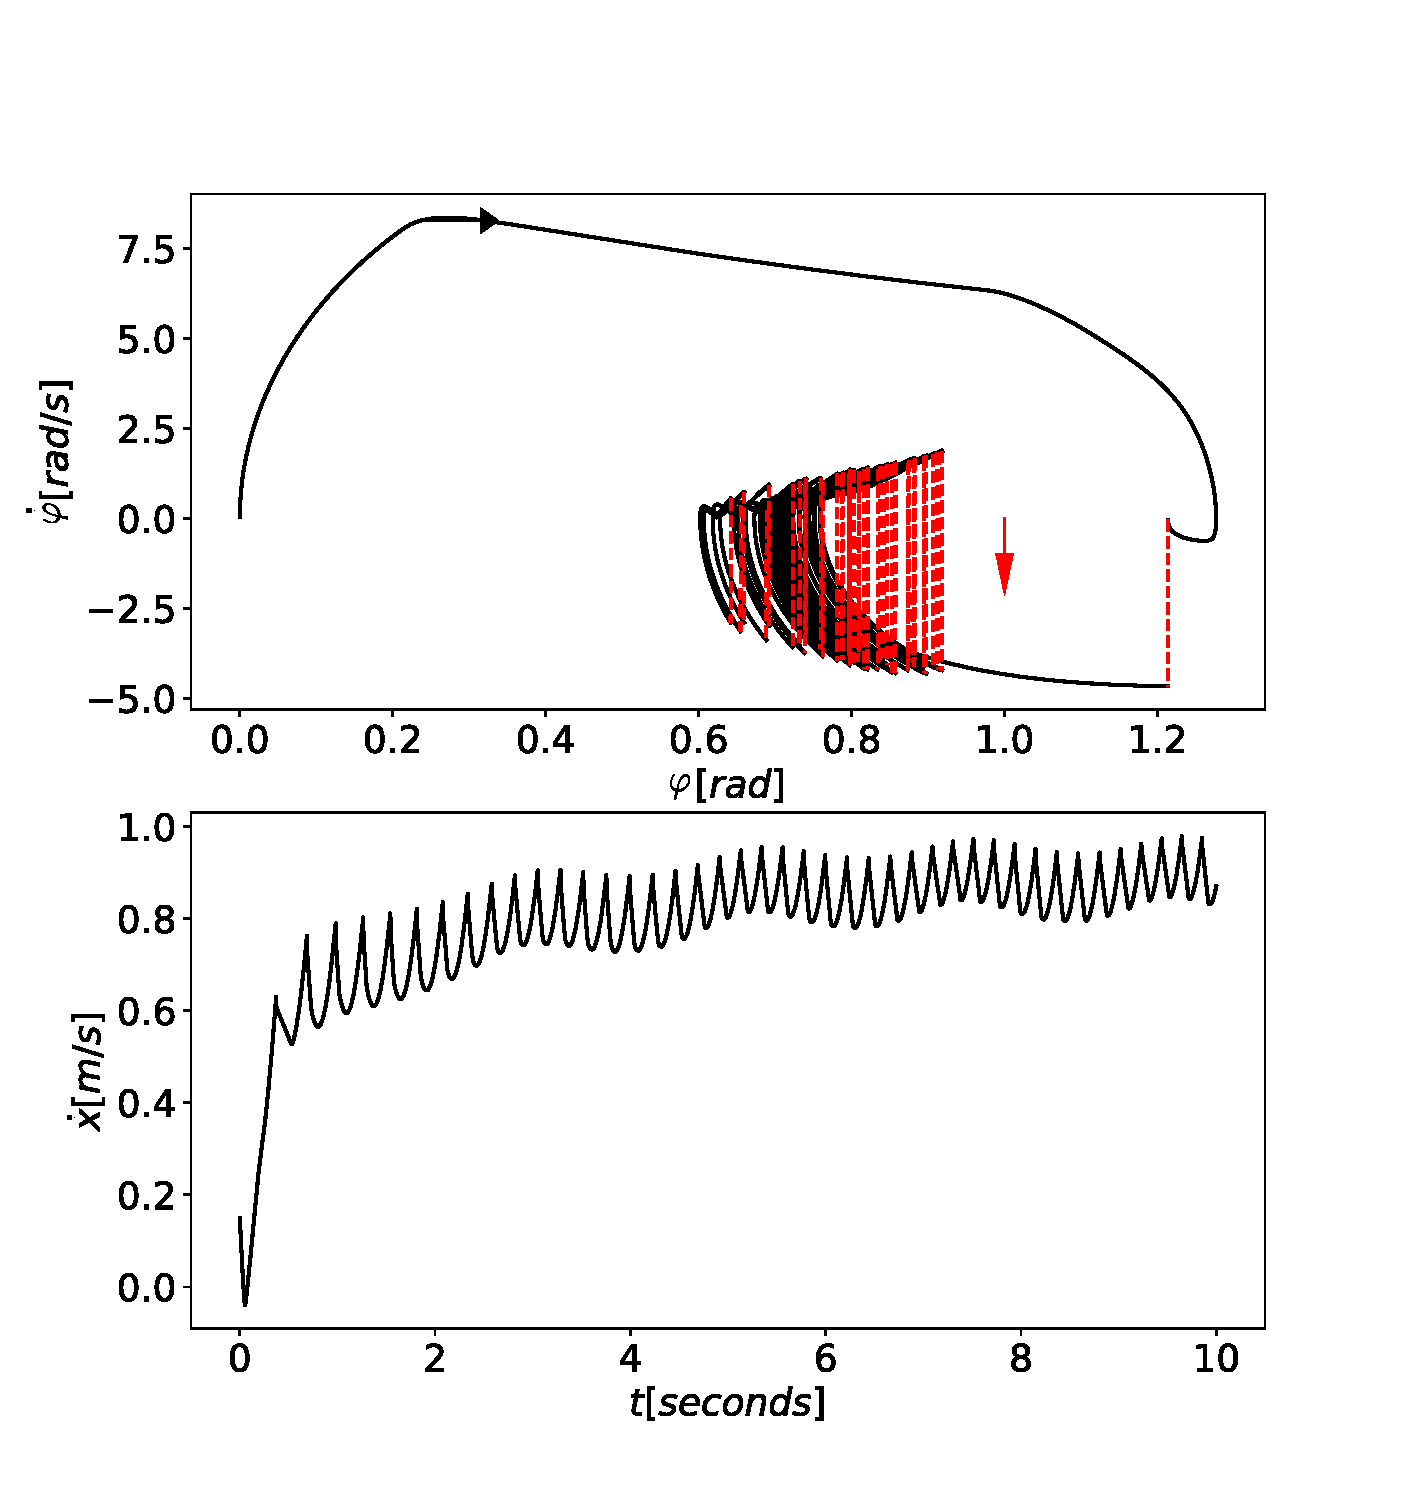
\includegraphics[width=0.8\columnwidth]{RW_deter_trajectory2.eps}
    \caption{Top: Torso orientation and velocity for 10-second trajectory. The
            solid black lines show the continuous phases and the dashed red
            lines show discrete transitions. Bottom: Horizontal hip speed}
    \label{fig:deter_rw_trajectory}
\end{figure}

\begin{figure}[H]
    \centering
    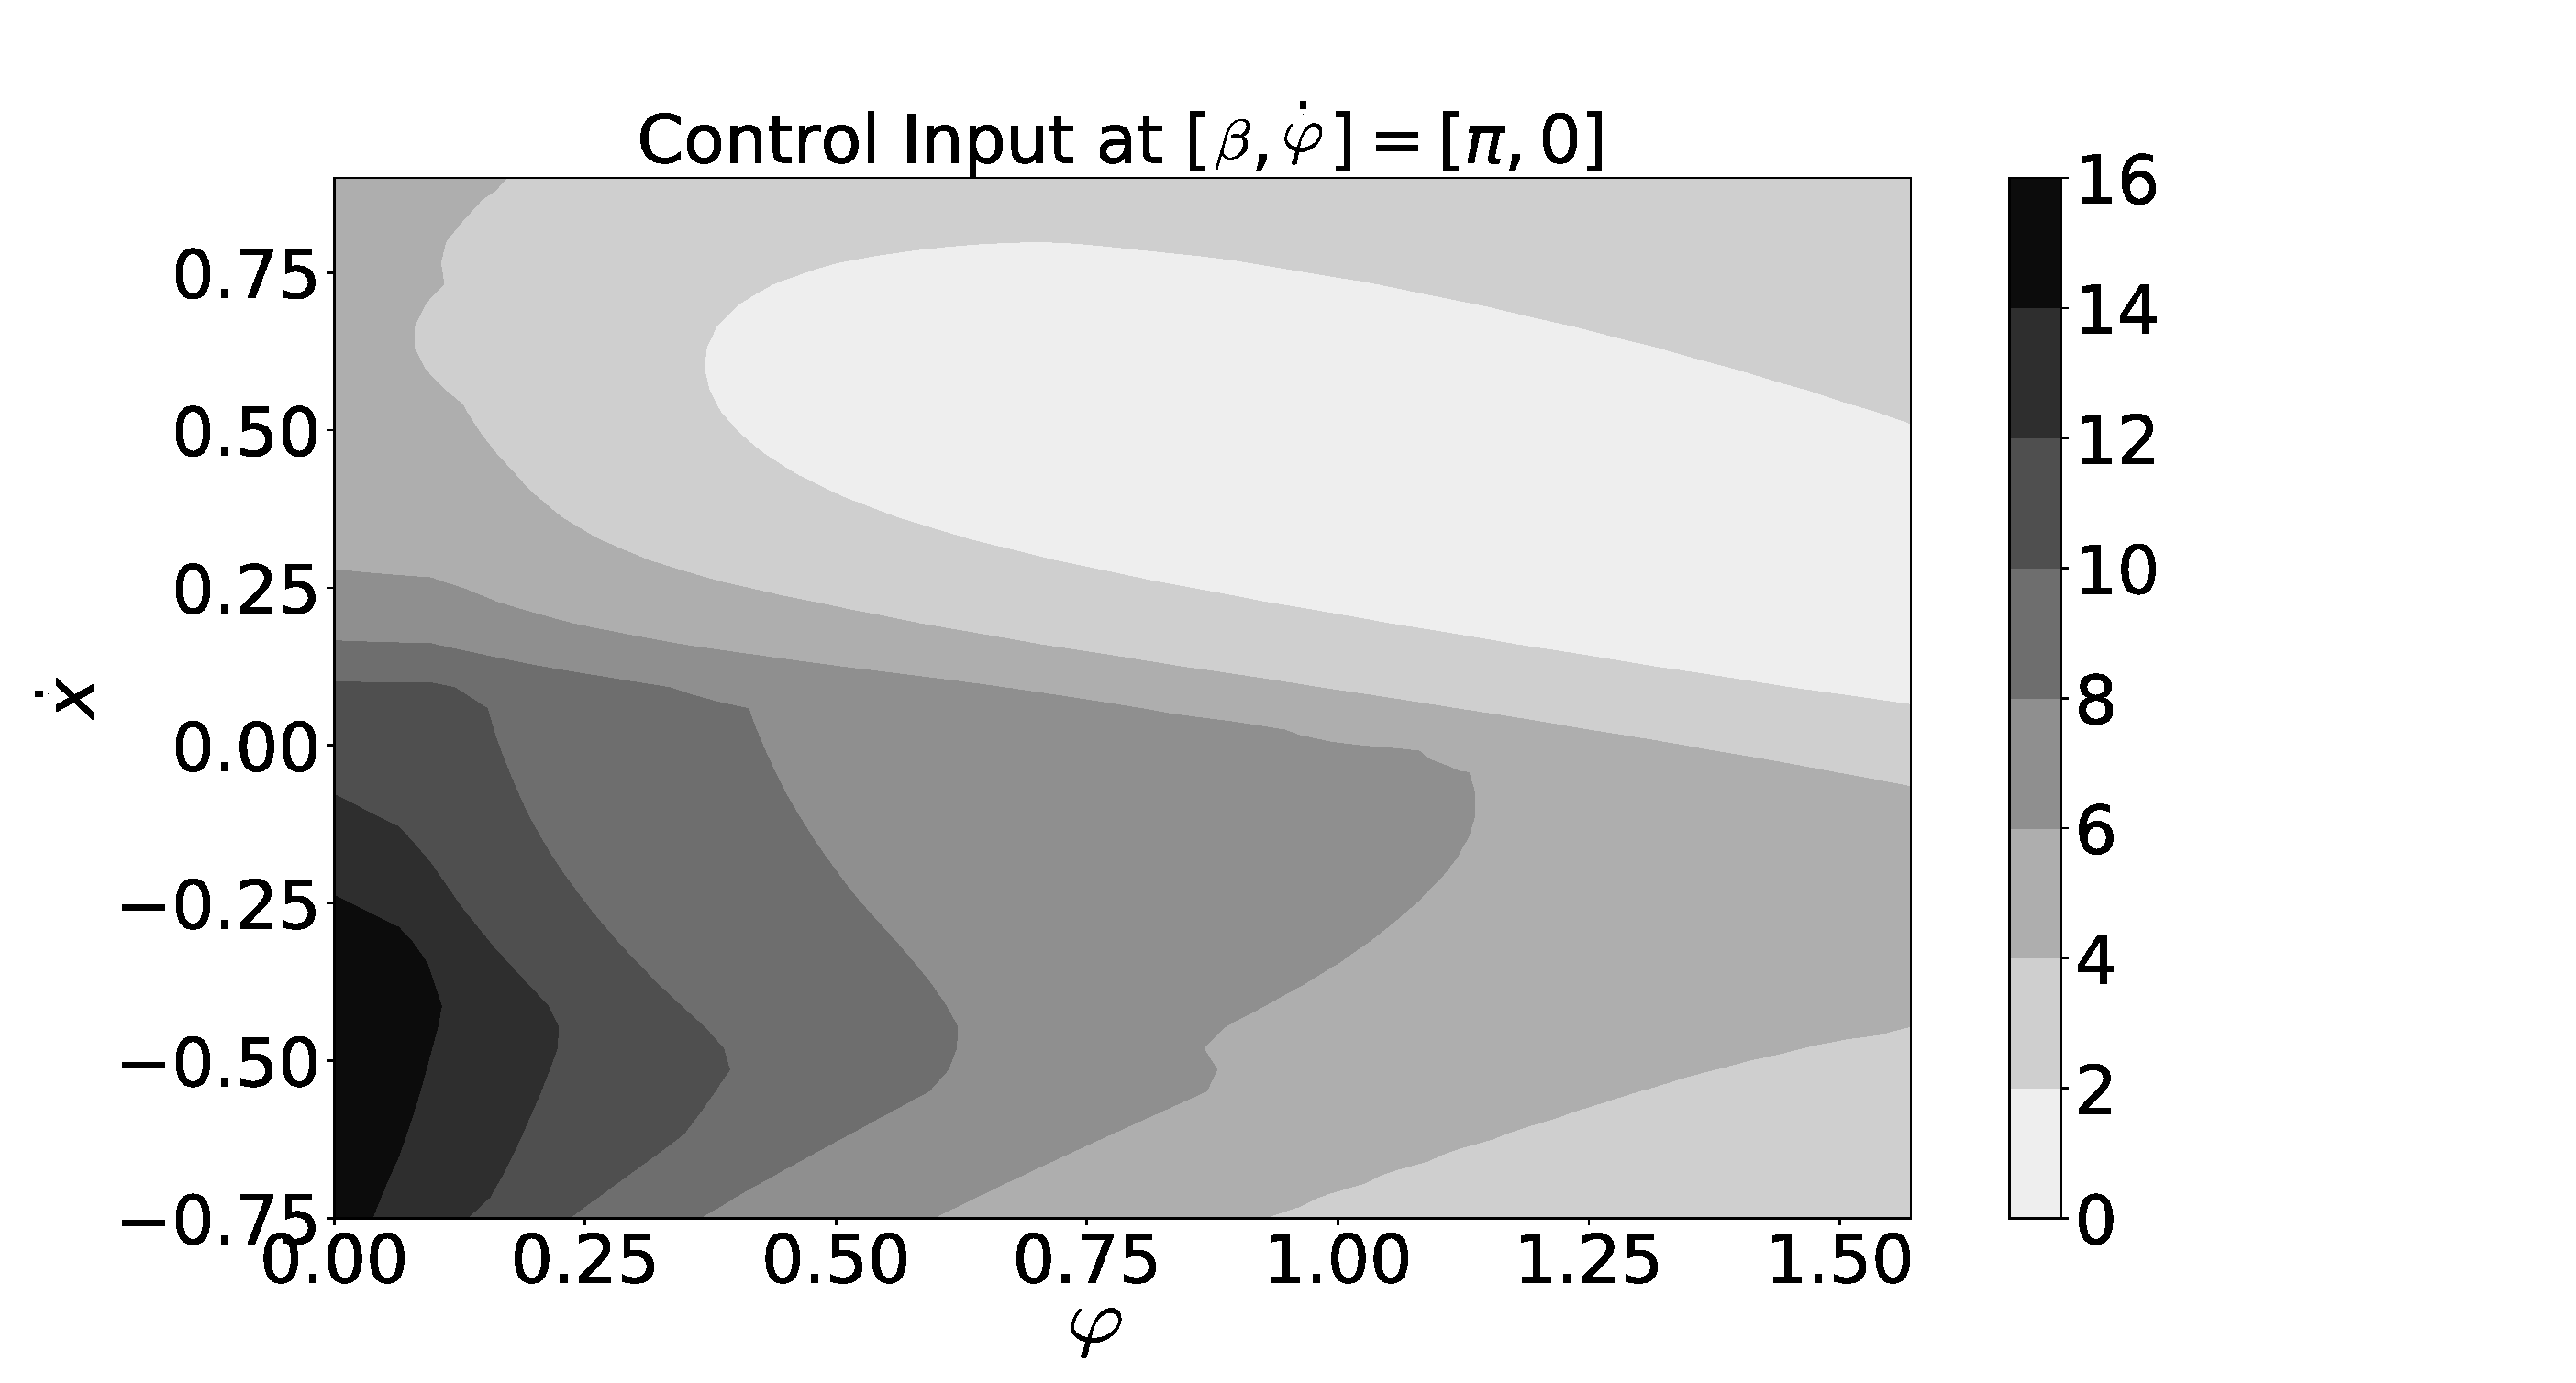
\includegraphics[width=0.9\columnwidth]{RW_deterministic_control2.eps}
    \caption{Torque command to torso as a function of torso angle and horizontal hip speed}
    \label{fig:deter_control}
\end{figure}
We compare the performance of the deterministic and Bayesian controllers as
follows.
%
Similar to the Bayesian training, we sample the terrain elevation from $p_s \sim
\mathbb{U}(0, p_{max})$ where $p_{max} = [0, 0.5, 1, 1.5, 2]$ centimeters.
%
As the value of $p_{max}$ increases, the difference in elevation between two consecutive 
spokes increases.
%
For instance, for $p_{max} = 0.5$, one spoke can be on a level ground and the adjacent spoke can be 
up to $0.5$ cm higher.
%
As $p_{max}$ increases to 2cm, the neighboring spokes can have up to 2cm
elevation difference, which requires a large torque to overcome the steep rise
in elevation.
% 
For each value of $p_{max}$, we generate 10 random initial states $x_0$ and
integrate 10-second-long trajectories.
%
The cost $J_T$ of each trajectory is calculated as per~\eqref{eq:loss}.
%
The bars in Figure~\ref{fig:comparison} show the average $J_T$ over the
10 trajectories for each $p_{max}$.
%
Notice that the Bayesian training consistently incurs less cost in all
elevation differences compared to its deterministic counterpart.
%
The deterministic training accumulates more cost with each increment in the
value of $p_{max}$, while the Bayesian training incurs a relatively consistent
cost across all values of $p_{max}$. 
%
This demonstrates the improved robustness properties of Bayesian
\textsc{NeuralPbc} under uneven terrain.

\begin{figure}[tb]
    \centering
    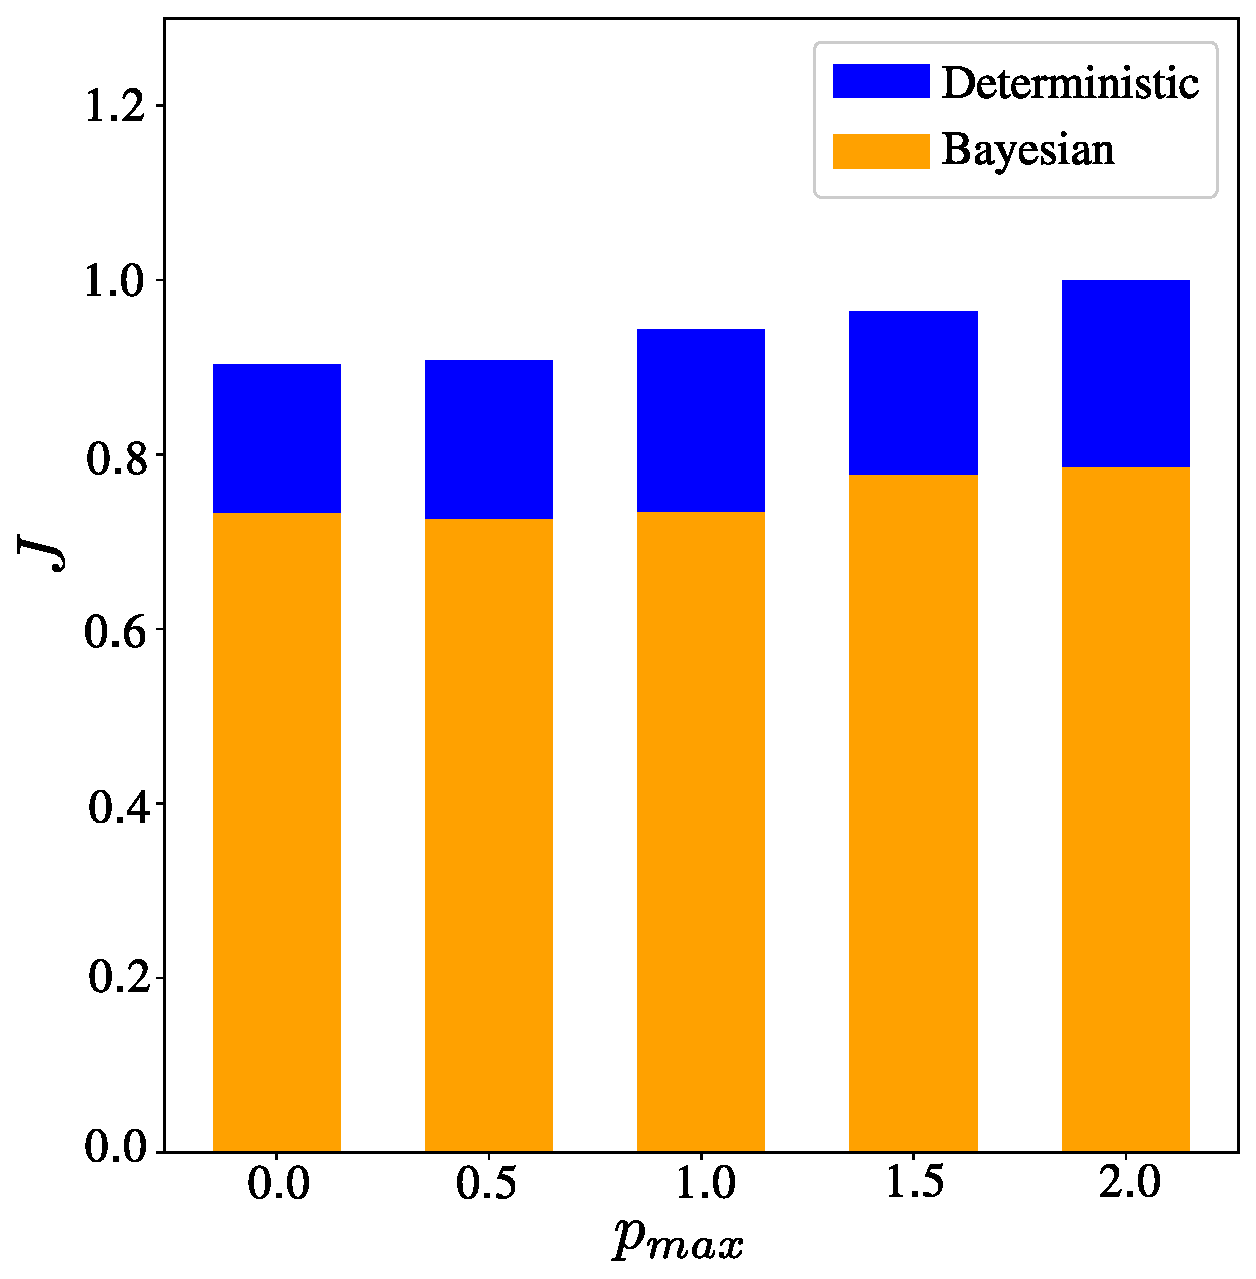
\includegraphics[width=0.6\linewidth]{simulationComparison.eps}
    \caption{Comparison of deterministic and Bayesian control for the rimless wheel.}
    \label{fig:comparison}
\end{figure}

\subsubsection{Real-World Experiments}

We test the performance of both the deterministic and Bayesian controllers on
the hardware shown in Figures~\ref{fig:hardware} and~\ref{fig:rw_picture}.
%
The robot consists of two set of $10$ spokes for stability.
%
The torso holds two ODrive v3.6 brushless DC motors, which actuate the drive
shaft through a belt-drive system.
%
The end of the Aluminum spokes land on preloaded springs to reduce vibration,
while the rubber feet ensure no-slip condition.
%
The incremental capacitive encoders attached to the motors report the
orientation of the spokes.
%
We use IMU readings fused with Mahony filter~\cite{mahony2008nonlinear} to estimate
the pitch of the torso.
%
A 24V battery pack is placed at the bottom edge of the torso to power
the motors, a Raspberry Pi 3B and a Teensy microcontroller.
%
We evaluate the neural networks on a laptop and exchange sensor readings and
torque commands with the Raspberry Pi via ROS wireless communication protocols.

Figures~\ref{fig:deter_even} and~\ref{fig:bayes_even} show the horizontal hip
speed achieved by the deterministic and Bayesian controllers, respectively, on
the hardware,
%
The real-world experiments exhibit very similar behavior to the simulation
results shown in Figure~\ref{fig:deter_rw_trajectory}.
%
Both controllers are able to reach and maintain the desired hip speed of the
walking machine.
%
Akin to the simulation results, both controllers periodically apply large torque
to react to the energy loss due to impacts.
%
Compared to the deterministic controller, the Bayesian controller exhibits spikes
in hip speed.
%
This is due to the marginalizing scheme, which randomly samples parameters
that result in a high torque in order to overcome large changes in elevation.
%
This behavior is very beneficial in preventing the mechanism from stumbling due
to impacts on uneven terrain. 

\begin{figure}[H]
    \centering
    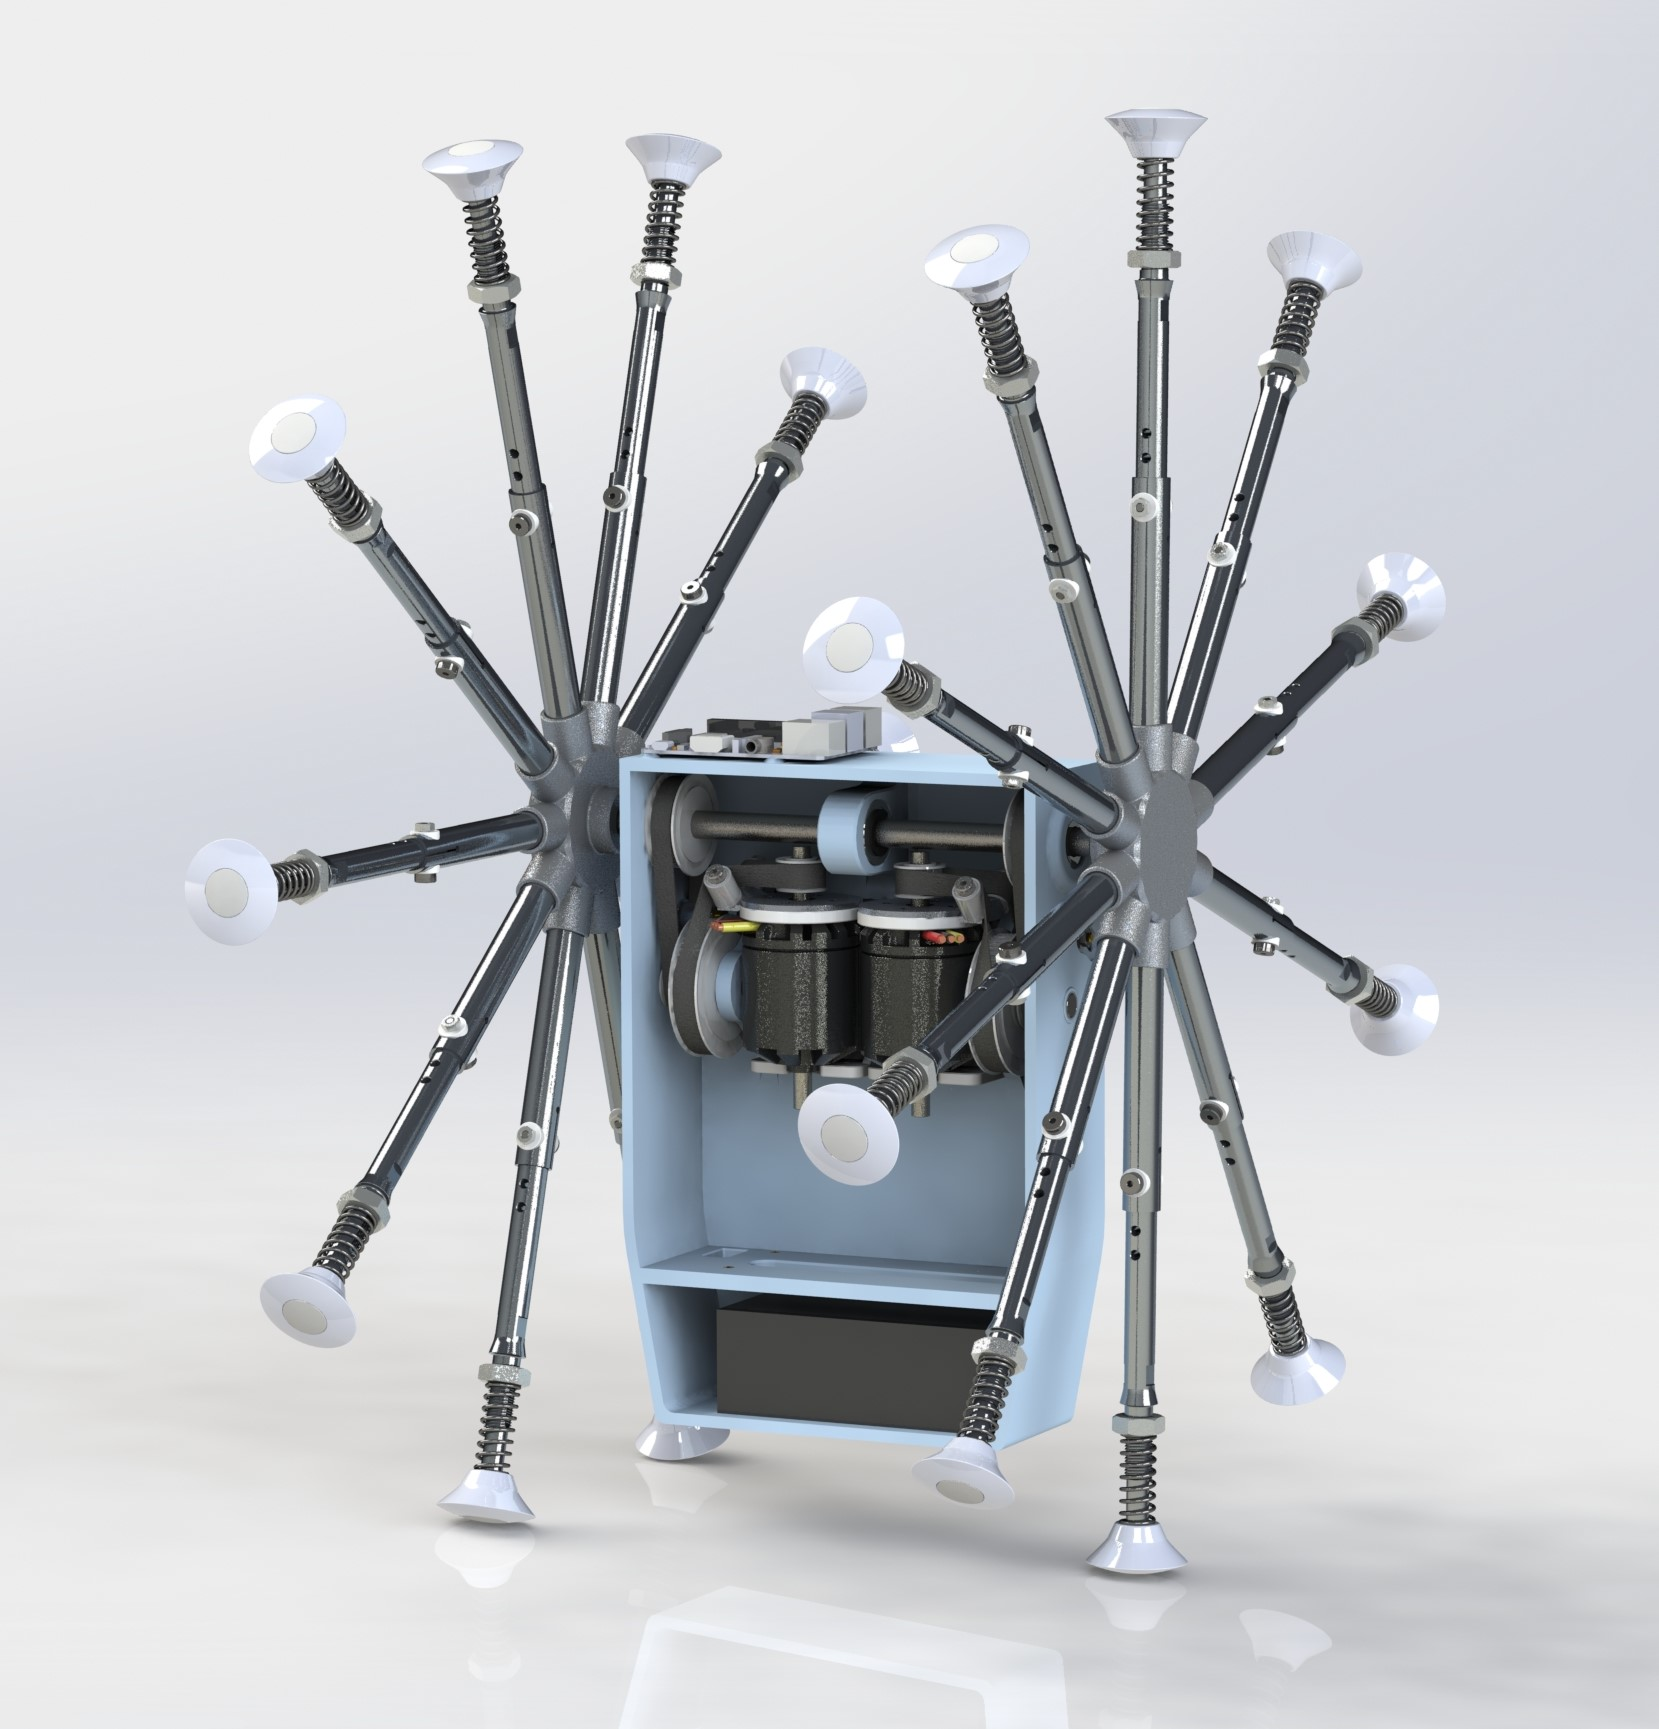
\includegraphics[width=0.5\columnwidth]{rendering.JPG}
    \caption{Rimless Wheel Assembly}
    \label{fig:hardware}
\end{figure}
\begin{figure}[H]
    \centering
    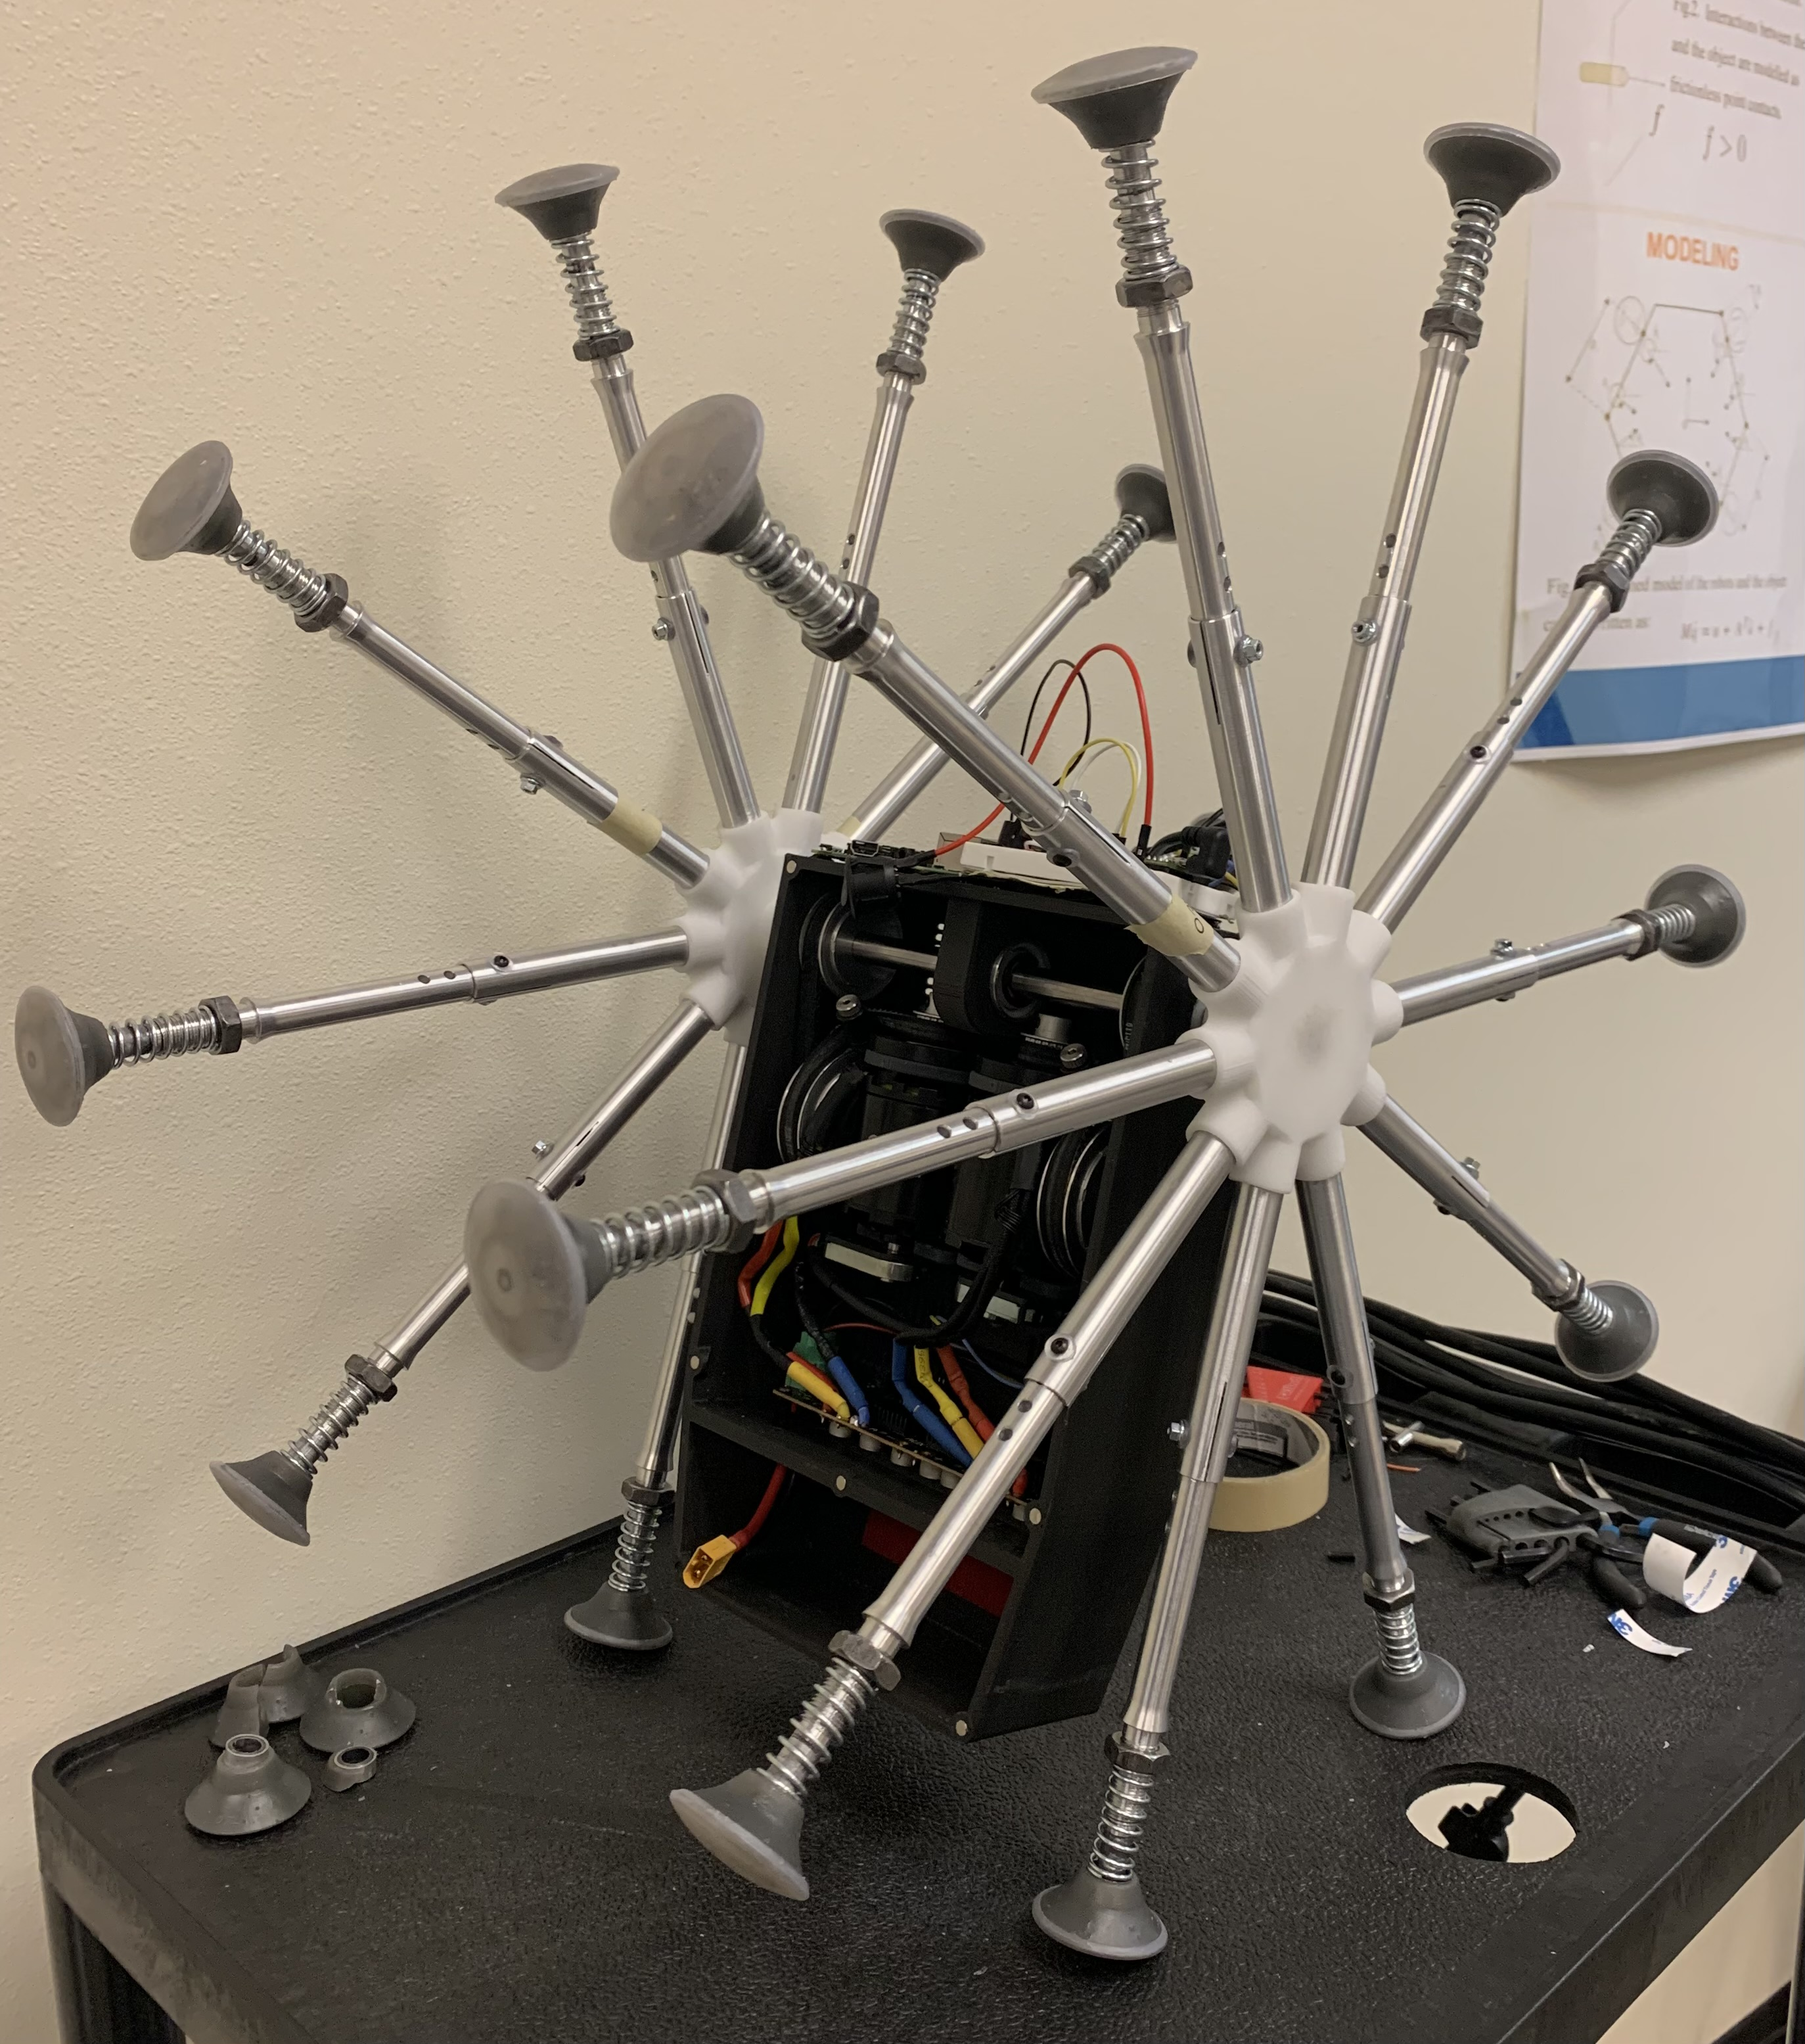
\includegraphics[width=0.5\columnwidth]{rimlesswheel_hardware.jpg}
    \caption{Rimless Wheel Hardware}
    \label{fig:rw_picture}
\end{figure}
\begin{figure}[H]
    \centering
    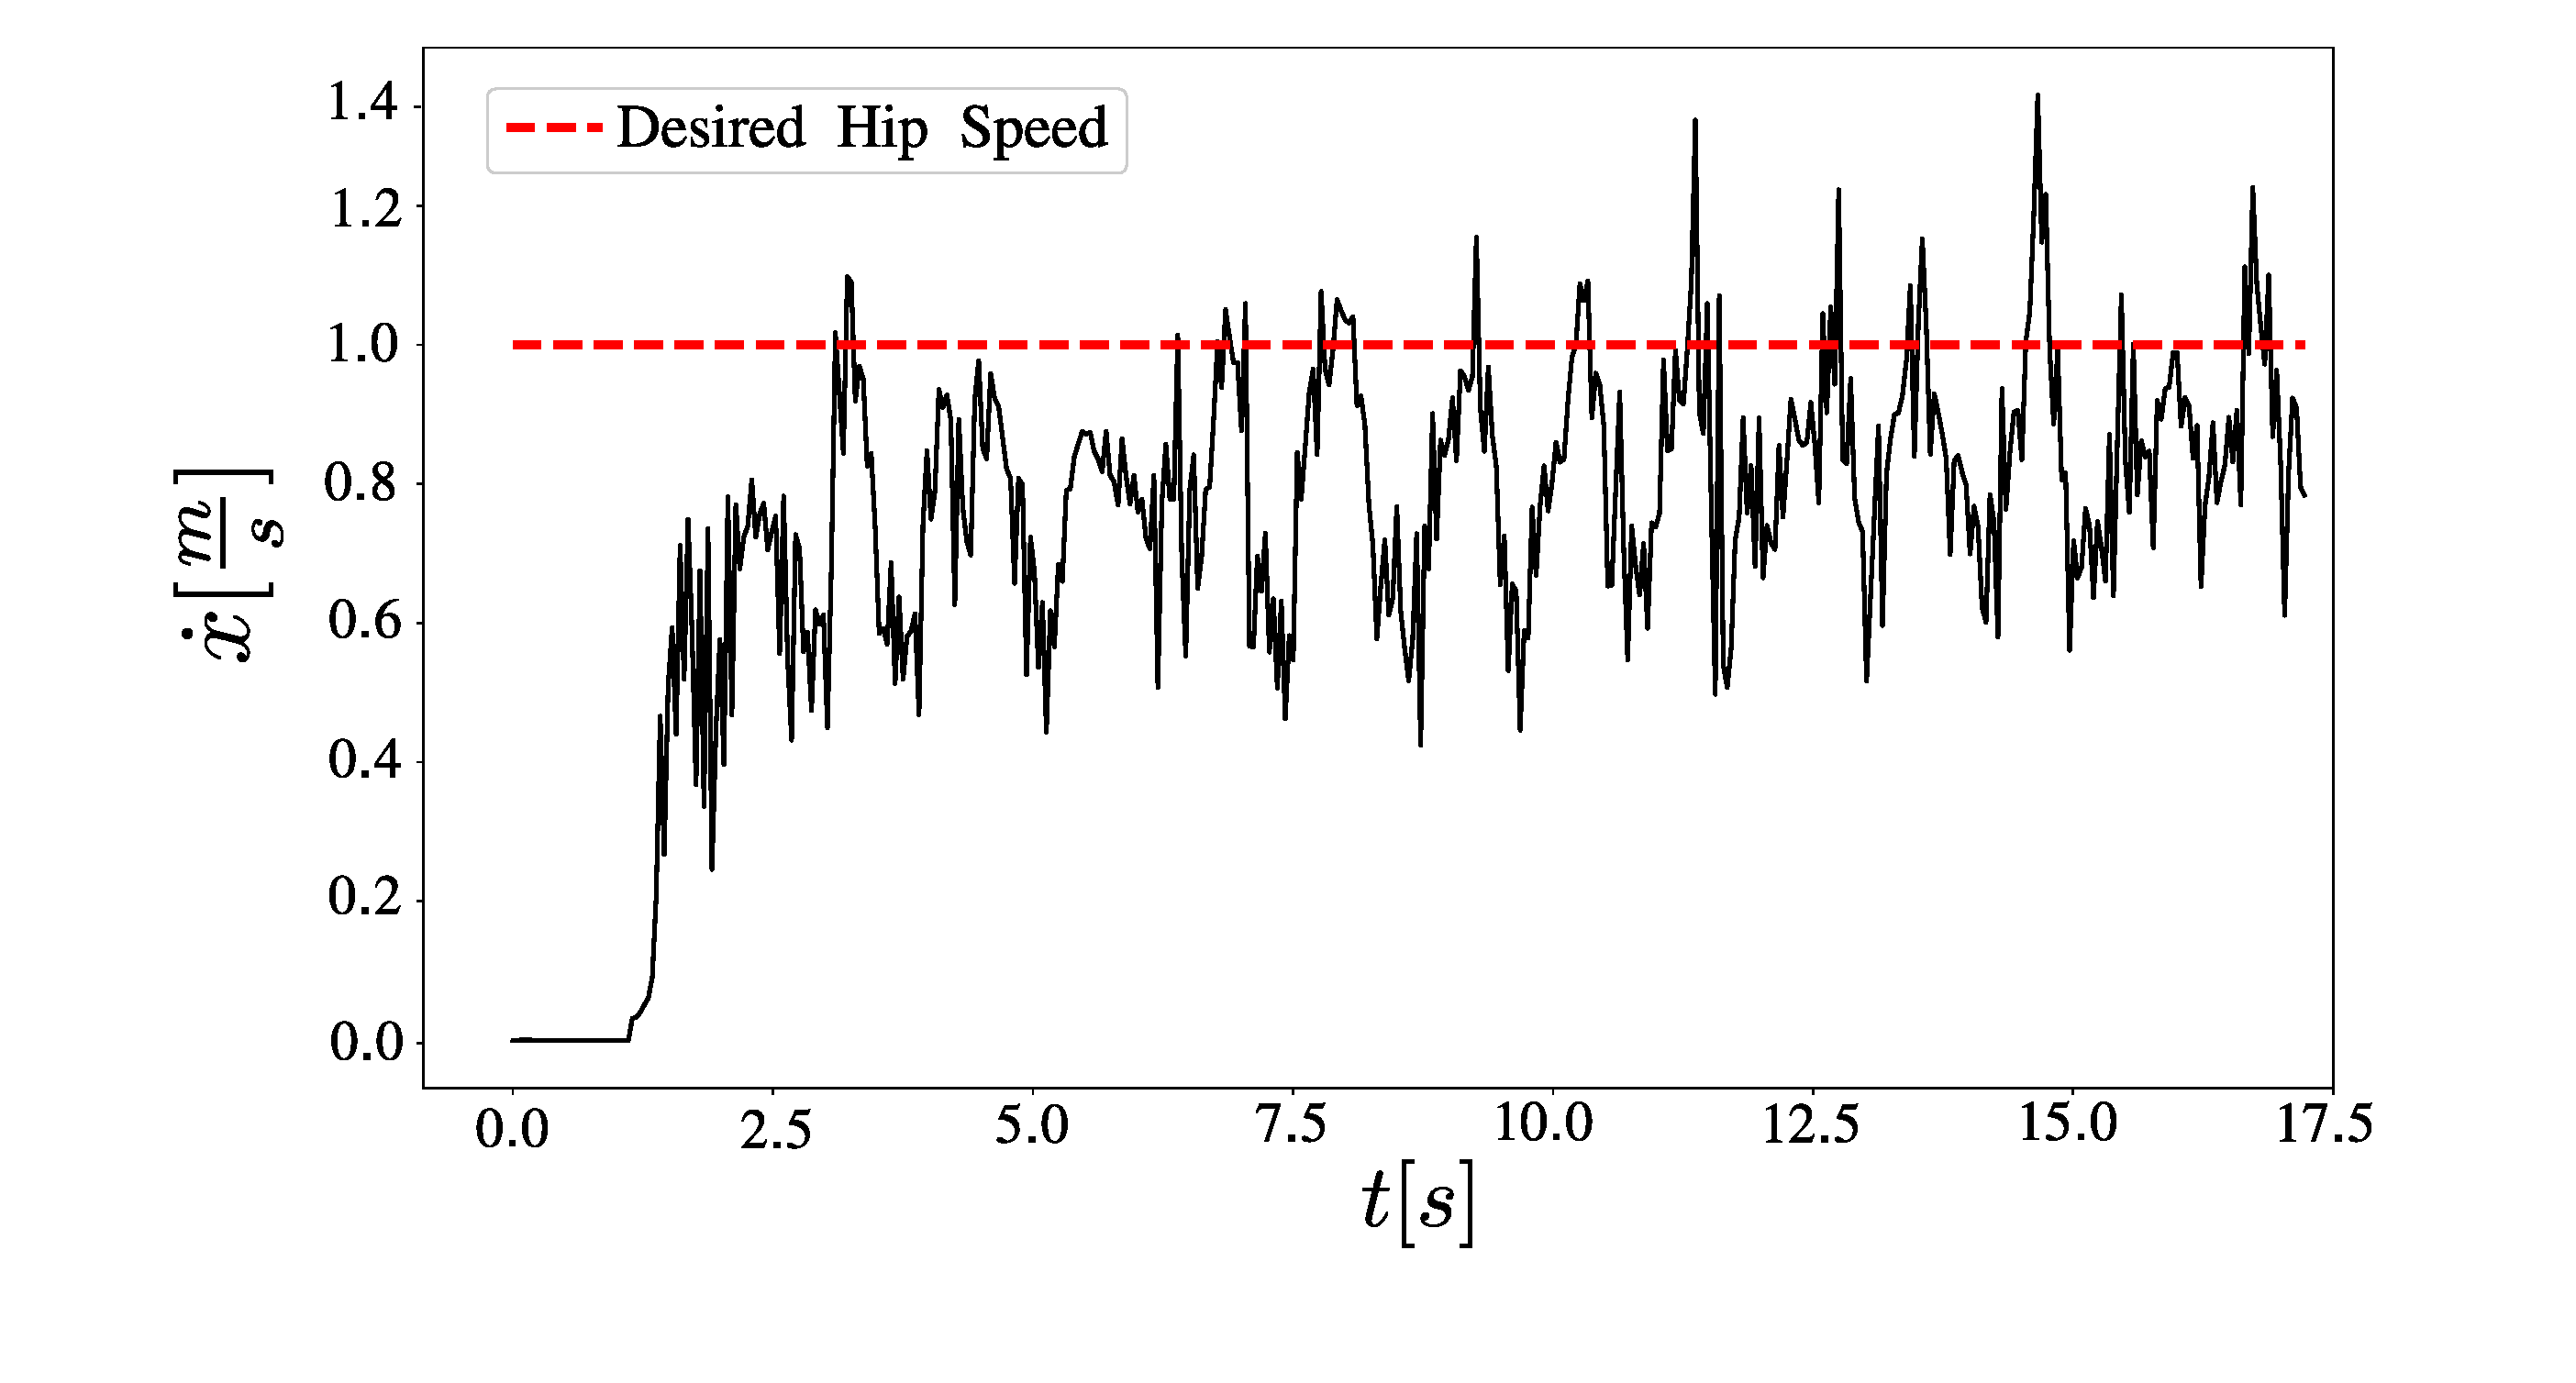
\includegraphics[width=0.7\columnwidth]{deter_even.eps}
    \caption{Trajectory generated by deterministic controller}
    \label{fig:deter_even}
\end{figure}
\begin{figure}[H]
    \centering
    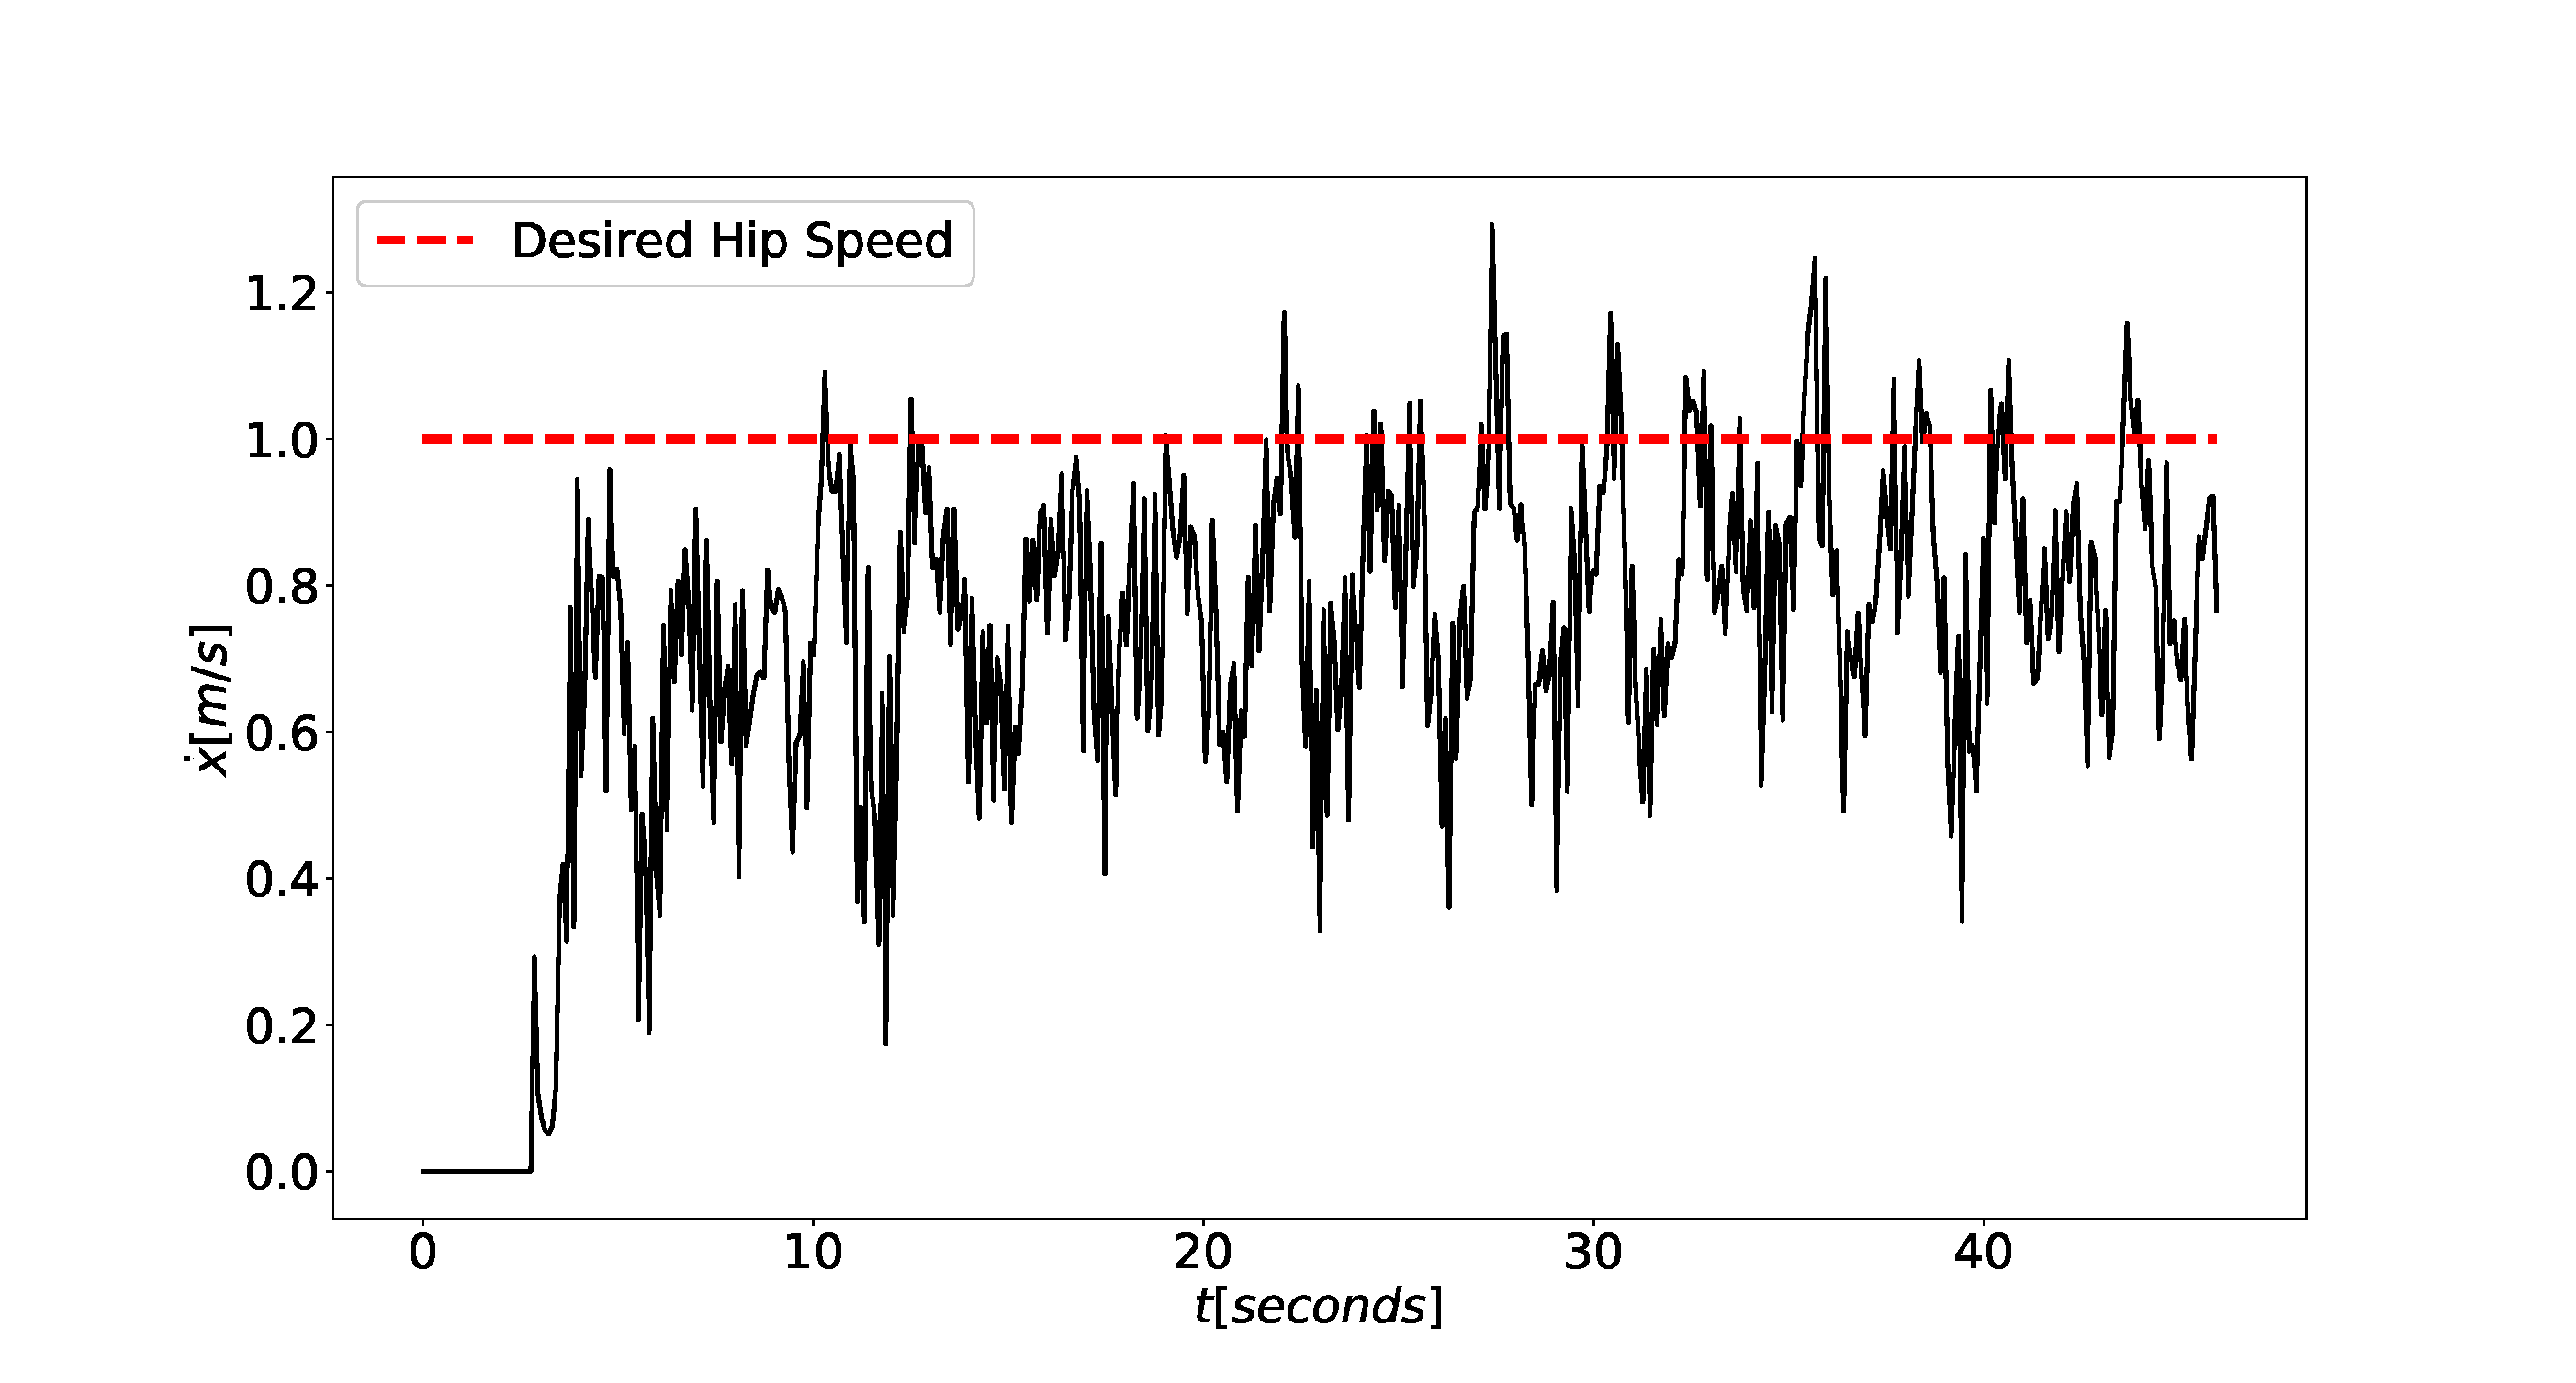
\includegraphics[width=0.8\columnwidth]{bayes_even.eps}
    \caption{Trajectory generated by Bayesian controller}
    \label{fig:bayes_even}
\end{figure}
%%%%%%%%%%%%%%%%%%%%%%%%%%%%%%%%%%%%%%%%%%%%%%%%%%%%%%%%%%%%%%%%%%%%%%%%%%%%%%%%%%%

\section{Bayesian Neural Interconnection and Damping Assignment PBC}

In this section, we validate the Bayesian \textsc{Neural-IdaPbc} framework on the
problem of swinging-up and stabilizing the inverted position of an inertia wheel
pendulum (IWP). 
%
We provide experimental results from simulation and real-world hardware in order
to thoroughly demonstrate the efficacy and robustness claims of Bayesian
inference.
\subsection{Inertia Wheel Pendulum}

The objective of this case study is to learn the parameters of $V_d, M_d, J_2$
that render the closed-loop passive and thus stable at the desired equilibrium
$x^*$, which corresponds to the upward position.
%
We utilize the system model provided in Section~\ref{subsec:iwp} to learn the decision
parameter $\theta$ from trajectories.
%
The optimization problem~\eqref{eq:idapbc_finite_optim} is constructed as
follows. 

\subsubsection{Training}

The potential energy function $V_d^\theta$ is a fully-connected neural
network with two hidden layers, each of which has the activation function
\textsc{Elu}.
%
The closed-loop mass matrix is constructed according to the Cholesky
decomposition $M_d^\theta = L^\top_\theta L_\theta$, where the components of
$L_\theta$ are part of the parameters $\theta$ to be optimized.
%
We choose $J_2^\theta = 0$, as the mass matrix is independent of $q$ for
this system.
%
The parameters of the surrogates are initialized according to the Glorot
(Xavier)~\cite{glorot2010understanding} scheme.
%
The optimization problem is solved over a uniform discretization of $q = \left(
q_1, q_2 \right) \in [-2\pi, 2\pi] \times [-50, 50]$.


In the deterministic setting, the nominal system parameters reported in
Table~\ref{tab:modified_params} are used for $H(q,p)$ during training. 
%
In the Bayesian setting, the standard deviations $\sigma_{p}$ of system
parameters $p_s = [I_1, I_2, mgl]$ are chosen to be $10\%$ of the nominal system
parameters given in Section~\ref{subsec:iwp}.
%
We use variational inference to estimate a Gaussian posterior distribution
over uncorrelated parameters.
%
After training, both settings use the nominal values for the computation of
$H(q,p)$ in the control synthesis given by Equation~\eqref{eq:idapbc_ues}.
%
A summary of the hyperparameters for both the deterministic and Bayesian methods
are given in Table~\ref{tab:training_setup_idapbc}. 
\begin{table}[t]
    \centering
    \caption{\textsc{Neural-IDAPBC} training setup for deterministic and Bayesian frameworks}
    % \rowcolors{2}{}{Wheat1}
    \begin{tabular}{lcc}
    \toprule
    %   & \multicolumn{2}{c}{Framework} \\
    %   \cmidrule(lr){2-3}
    & Deterministic & Bayesian \\
    \midrule
        Neural net size & (2, 8, 4, 1) & (2, 8, 6, 1)\\
        \# of parameters &  56  & 150\\
        Optimizer & \textsc{Adam} & DecayedAdaGrad\\
        Initial learning rate & 0.001 & 0.01\\
    \bottomrule
    \end{tabular}
    \label{tab:training_setup_idapbc}
\end{table}

\subsubsection{Simulation Tests} 
The performance of the controllers obtained from the deterministic and Bayesian
trainings are compared as follows.
%
% Both frameworks are trained with the nominal system parameters given in
% Table~\ref{tab:modified_params}.
%
Similar to the \textsc{NeuralPbc} simulation tests, we introduce system
parameter uncertainties by moving the average system parameters by $\pm
10\%$ to $\pm 50\%$ with increments of $10\%$. 
%
For each average system parameter, we sample uniformly with a $\pm 5\%$ support
around the average system parameters. 
%
This helps test the performance of the controller with various combinations of
$I_1, I_2$ and $m_3$.
%
%
% On top of the system parameter uncertainties, we introduce measurement noise
% represented by a Wiener process with standard deviation of $0.005$ and $0.05$ on
% the joint angles and velocities, respectively. 
%
Figure~\ref{fig:comparison_idapbc} shows the performance of the controllers.
The policy learned from the Bayesian training is marginalized over 10
parameters sampled from the posterior per~\eqref{eqn:marginalization}.

As seen in Figure~\ref{fig:comparison_idapbc}, trajectories from the Bayesian
controller incur much lower cost than the deterministic counterpart throughout a
wide range of errors in system parameters.
%
Moreover, we observe that the error band on the cost corresponding to Bayesian
training is narrower.
%
These results show that controllers trained via Bayesian learning are
consistently more robust to errors in system parameters.
\begin{figure}[tb]
    \centering
    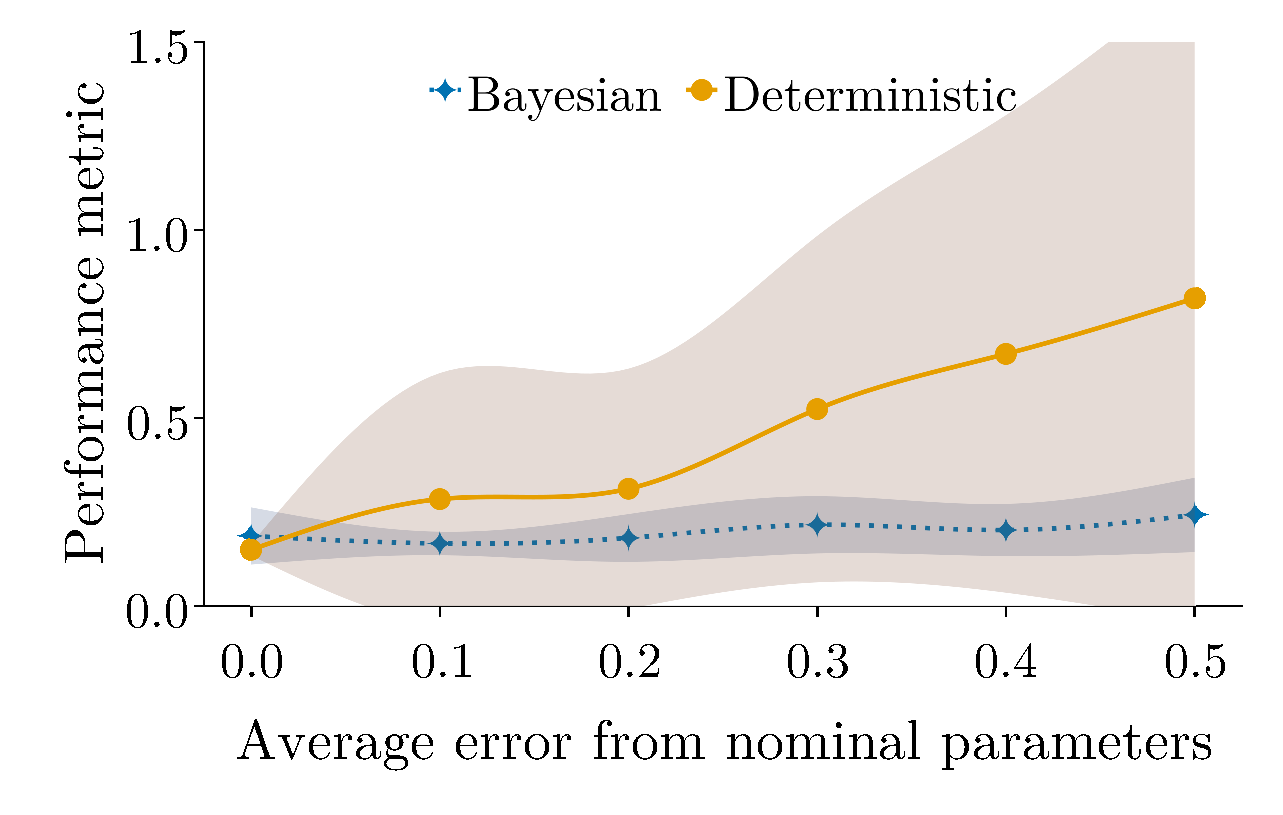
\includegraphics[clip,width=0.7\columnwidth]{./figures/bandplot1.eps}%
    \caption{
        %
        Accumulated quadratic cost ($J^T$) for a range of error in system
        parameters. 
        %
        Lower values correspond to better controller performance.
        %
    }
    \label{fig:comparison_idapbc}
\end{figure}

\subsubsection{Hardware Tests} 

The hardware experiments are designed to further demonstrate the robustness of our
controllers against model uncertainties, which include errors in the parameters,
friction in the bearings, and any contribution to the dynamics from the
belt-drive system.
%
We deliberately modify the hardware to create large errors in the model
parameters and test the controllers without any additional training.
%
In particular, the inertia wheel attached to $q_2$ is replaced with parts whose
mass and inertia values differ from the nominal values (see
Table~\ref{tab:modified_params}). The state $x$ is recorded, and the performance
metric~\eqref{eq:performance_metric} is used to evaluate the controllers.
%
The results are summarized in Figure~\ref{fig:neuralidapbc_bar_plot}.

In all scenarios, we recorded a 100\% success rate in the swing-up task despite
the errors introduced in the system parameters.
%
Furthermore, we observe that the controller from Bayesian training consistently
outperforms the deterministic counterpart, supporting the
theoretical justification discussed in Section~\ref{sec:bl_justification}. 
\begin{figure}[H]
    \centering
    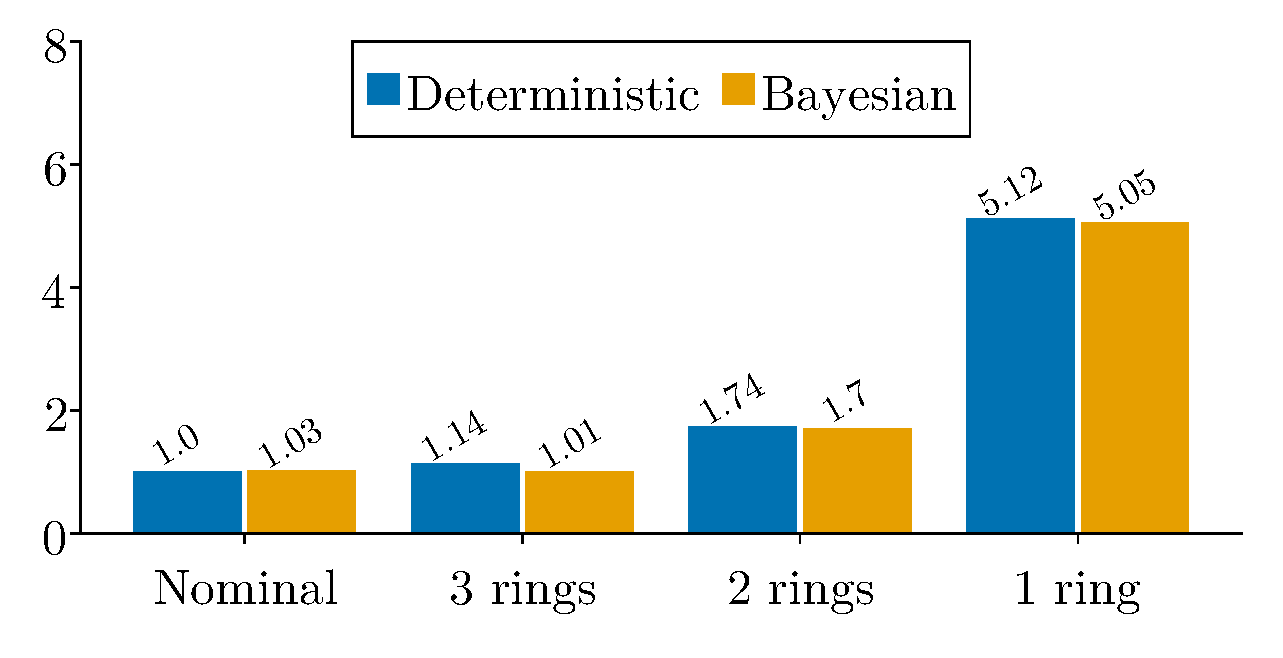
\includegraphics[width=0.7\linewidth]{./figures/idapbc_bar.eps}
    \caption{
        %
        Normalized accumulated cost $J_{T}$ (lower is better) for
        modified system parameters.
        %
        The categories A-C correspond to the parameters shown in
        Table~\ref{tab:modified_params}.
        %
    }
    \label{fig:neuralidapbc_bar_plot}
\end{figure}
%

